\documentclass[12pt,a4paper]{report}
\usepackage[bookmarks,unicode,hyperfootnotes=false]{hyperref}
\usepackage[utf8]{inputenc}
\usepackage[T1]{fontenc}
\def\magyarOptions{defaults=prettiest,mathmuskips=latex}
\usepackage[english,magyar]{babel}
\usepackage[paper=a4paper,left=3.5cm,right=2.5cm,top=2.5cm,bottom=2.5cm]{geometry}
\usepackage{amsmath}
\usepackage{amsfonts}
\usepackage{amssymb}
\usepackage{amsthm}
\usepackage{mathtools}
\usepackage{graphicx}
\usepackage{esdiff}
\usepackage{lmodern}
\usepackage{setspace}
\usepackage{indentfirst}
\usepackage{titlesec}
\usepackage{enumitem}
\usepackage[backend=biber,style=numeric,sortlocale=hu,babel=other]{biblatex}
\usepackage[autostyle]{csquotes}
\addbibresource{bibliography.bib}

\usepackage{comment}

\pdfinfo{
   /Author (Vadas Norbert)
   /Title (Robotkarok problémája)
   /Subject (matematika)
   /Keywords (alkalmazott; matematika; BSc; szakdolgozat; robotkarok)
}

\pagestyle{plain}
\frenchspacing
\onehalfspacing

\newtheorem{tét}{Tétel}[section]
\newtheorem{lem}[tét]{Lemma}
\newtheorem{áll}[tét]{Állítás}
\newtheorem*{köv}{Következmény}
\theoremstyle{remark}
\newtheorem*{megj}{Megjegyzés}
\theoremstyle{definition}
\newtheorem{defi}{Definíció}[section]
\newtheorem{pl}{Példa}[section]

\begin{document}
\titleformat{\chapter}[hang]
    {\normalfont\LARGE\bfseries}{\thechapter.}{1em}{}

\begin{titlepage}
\begin{center}
{\LARGE \textsc{Eötvös Loránd Tudományegyetem \\ Természettudományi Kar \\}}
\hrulefill \\[2.5cm]
{\huge Vadas Norbert} \\[0.7cm]
{\Huge \textsc{Robotkarok problémája}} \\[0.7cm]
matematika BSc szakdolgozat \\[0.1cm]
alkalmazott matematikus szakirány \\[2.2cm]
{\large Témavezetõ:} \\[0.4cm]
{\Large Szeghy Dávid} \\[0.3cm] 
{\Large Geometriai Tanszék}
\vfill

\includegraphics[width=0.3\textwidth]{./images/elte_cimer_ff}~\\[0.5cm]
{\large Budapest, 2013}
\end{center}
\end{titlepage}

\chapter*{Köszönetnyilvánítás}
\pagenumbering{roman}
Ezúton szeretném megköszönni témavezetőmnek, Szeghy Dávidnak, hogy megismertette velem ezt a remek témakört, hogy 
segített megoldani a felmerülő problémákat, valamint hogy figyelemmel kísérte és hasznos tanácsaival segítette a 
dolgozat megírását.

Köszönettel tartozom még minden gimnáziumi és egyetemi tanáromnak, akik megszerettették velem a matematikát, és 
bevezettek ennek a csodálatos tudománynak a rejtelmeibe.

Végül, de nem utolsósorban köszönöm menyasszonyomnak, Halmai Boglárkának a türelmét, a lelkesítését és minden 
támogatását, amelyet az elmúlt időszakban nyújtott, beleértve a nyelvtani és formai hibák javítását.

\tableofcontents

\chapter{Bevezetés}
\pagenumbering{arabic}
Mindenki hallott már robotokról, és mindenkiben él egy elképzelés arról, hogy ez a szó mit is takar valójában. 
Egyesek emberi kinézetű, intelligenciával rendelkező mechanikus lényeket neveznek így, mások egyszerű, automatizált 
eszközökre használják ezt a kifejezést. Akárhogyan is gondolunk rájuk, van bennük valami különleges, ami magával 
ragadja az ember fantáziáját. Nem csoda, hogy megannyi könyv és film született már ebben a témában.

Ebben a dolgozatban ipari robotokról, más néven robotkarokról lesz szó. Ezek az eszközök szegmensek és ízületek 
láncolatából állnak, és típusuktól függően többé-kevésbé az emberi karra hasonlítanak. Az itt említett fogalmakat a 
következő fejezetben fogjuk pontosan definiálni, valamint majd néhány példát is láthatunk a legelterjedtebb 
robotkar-konfigurációkra.

Az általános szemléletnek megfelelően ezek a robotok kiválóan alkalmasak a monoton, ismétlődő munkafolyamatokban 
az emberi tevékenység kiváltására. A tömeggyártásban elengedhetetlen a használatuk, mivel képesek nagy mennyiségű, 
közel azonos minőségű áru gyors, önálló előállítására. További előnyeik még az alacsonyabb előállítási költségek és 
a nagyobb precizitás. A robotkarok programozása azonban nem egy egyszerű feladat. Egy sor különféle, természetes 
módon felbukkanó problémára kell gyorsan kiszámítható megoldást adnunk. A továbbiakban néhány ilyen feladatot fogunk 
alaposabban is megvizsgálni.

A robotgeometriának vannak más alkalmazásai is. Az elmúlt évek technológiai fejlődése lehetővé tette, hogy egyre
élethűbb számítógépes animációkat készítsünk, akár filmekhez, akár videojátékokhoz. Ehhez az élethűséghez a puszta
látvány azonban nem elég: az is fontos, hogy a karakterek mozgása természetes, emberi legyen. Robotkarok 
használatával egyszerűen tudunk végtagokat matematikailag ábrázolni. Ezáltal az itt elért eredmények 
felhasználhatóvá válnak a digitális modellezésben is. Ennek megfelelően az előbb említett probléma megoldásában  
többek közt az inverz sebességkinematika fog segítséget nyújtani nekünk.

\section{Felhasznált ismeretek és jelölések}
A továbbiakban elsősorban geometriai és lineáris algebrai ismeretekre lesz szükségünk, melyek megtalálhatóak 
\az+\textcite{hajos_geo}, illetve \az+\textcite{freud_linalg} könyvekben. Ezen eredményeket nem fogjuk részletezni, 
hanem már ismertnek tekintjük őket.

A dolgozat nagymértékben támaszkodik \az+\textcite{spong_robot} könyv ide vonatkozó fejezeteire, mind tartalmilag, 
mind a felhasznált képek, illetve jelölések tekintetében. Ennek megfelelően a mátrixokat nagybetűvel, a vektorokat 
és skalármennyiségeket kisbetűvel jelöljük, a koordináta-tengelyeket pedig gyakran azonosítjuk a hozzájuk tartozó 
bázisvektorokkal. Ezenfelül az indexek használatát illetően a következőképpen járunk el. A felső index mindig a 
referencia koordináta-rendszert jelöli, vagyis azt a rendszert, amelyben a mennyiséget felírtuk. Az alsó index azt a 
rendszert jelöli, amelynek az adott mennyiségét kifejeztük a referencia-rendszer szerint. Tehát az $R^{i}_{j}$ 
forgatási mátrix a $j$ rendszer elfordulását adja meg az $i$ rendszerhez képest, az $o^{i}_{j}$ vektor pedig a $j$ 
rendszer origóját adja meg az $i$ rendszer koordinátáival. Az $\omega$ szögsebesség-vektorok esetében az alsó két 
index azt jelöli, hogy mely két rendszer közötti elfordulás szögsebességét írjuk le a referencia-rendszerben. 

Ezen kívül deriválás alatt mindig a $t$ időparaméter szerinti deriválást értjük, és a változó fölé írt ponttal vagy 
$\diff{}{t}$-vel jelöljük. Továbbá az egyszerűség kedvéért gyakran el fogunk hagyni bizonyos indexeket és változókat 
mindaddig, amíg ebből nem zármazik félreértés. Legtöbbször ez a $t$ időparamétert és a bázisrendszerre vonatkozó $0$ 
indexet érinti.

\chapter{A robotgeometria alapjai}
Ahhoz, hogy robotkarokkal tudjunk dolgozni, szükségünk lesz egy matematikai modellre, amely segítségével könnyen 
leírhatóvá és kezelhetővé válnak a felmerülő problémák. Ebben a fejezetben ezt a modellt fogjuk felépíteni. Először 
is definiálnunk kell, mi is az a robot.

\begin{defi}[A Robot Institute of America szerint]
A robot egy újraprogramozható, többfunkciós manipulátor anyagok, eszközök, részegységek vagy speciális műszerek 
változókkal programozott mozdulatsor segítségével való mozgatására tervezve, különféle feladatok elvégzése 
érdekében.
\end{defi}

Ebben a definícióban a kulcsfogalom az újraprogramozhatóság. A számítógépes vezérlés adja a robotok 
használhatóságát és alkalmazkodóképességét. Léteznek ugyanis úgynevezett teleoperátorok, melyek folyamatos emberi 
irányítást igényelnek. Ezeket nem soroljuk a robotok közé.

\begin{figure}[b]
\centering
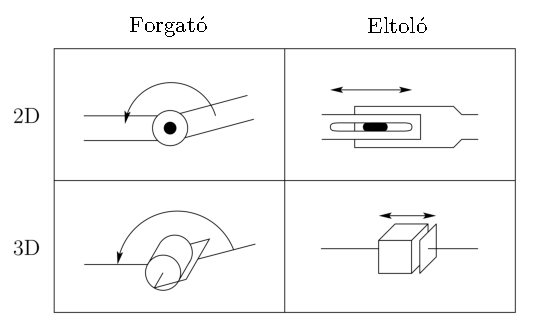
\includegraphics[width=0.6\linewidth]{./images/Joint_types}
\caption{Forgató és eltoló ízületek kettő és három dimenzióban}
\end{figure}

Felépítését tekintve a manipulátor merev testek, szegmensek sorozata, amelyek ízületekkel vannak összekötve. Ezek 
egy kinematikai láncot alkotnak, amelynek végén valamilyen szerszám található, amelyet kéznek nevezünk. A robotkar 
munkatere azon térbeli pontokból áll, amelyekbe a kéz eljuttatható. A kinematikai láncot nyíltnak nevezzük, ha a két 
végét csak egy szegmens-sorozat köti össze; ellenkező esetben zárt láncról beszélünk. Az ízületek típusuk szerint 
lehetnek forgatók (revolute, R) vagy eltolók (prismatic, P). Ezeket elemi, egy szabadságfokú ízületeknek hívjuk.  
Mivel bármely több szabadságfokú ízület előáll elemi ízületekből, így nem jelent megkötést csak ezekkel foglalkozni.

A nyílt láncú robotkarokat a ízületek típusának felsorolásával adjuk meg, a bázistól a kéz felé haladva, pl.: RRP. A 
forgató ízületek egy tengely körüli forgatást, az eltoló ízületek egy tengely menti eltolást valósítanak meg. Ezt a 
tengelyt az adott ízület hatástengelyének nevezzük. Könnyen látható, hogy minden ízület állapota megadható egyetlen 
paraméterrel: az elfordulás szögével vagy az eltolás mértékével. Ezeknek a $q = (q_1, \ldots, q_n)$ vektorát a 
manipulátor egy konfigurációjának nevezzük. A paraméterek, vagyis az ízületek számát a robotkar szabadságfokának 
hívjuk.

A paraméterekkel kapcsolatban kétféle probléma fogalmazható meg, a direkt és az inverz kinematikai probléma. Az 
előbbinél adottak az ízületi paraméterek, és a cél a kéz helyzetének a meghatározása, az utóbbinál pedig a kéz 
helyzete ismert, és keressük az azt megvalósító paramétereket. A következőkben ezekkel a problémákkal fogunk 
foglalkozni, de előbb még lássunk néhány példát a legelterjedtebb robotkarokra.

\section{Példák robotkarokra}
Habár számtalan módon lehetséges forgató és eltoló ízületek segítségével különféle kinematikai láncokat létrehozni, 
a gyakorlatban ezek közül csak néhány speciális konfiguráció használata az elterjedt. Most ezek közül mutatunk be 
hármat.

\subsection{Az antropomorf robotkar (RRR)}
Az antropomorf, más néven humanoid robotkar három forgató ízületből áll. Ezek közül a második és a harmadik ízület 
hatástengelyei párhuzamosak egymással, és merőlegesek az első ízület hatástengelyére. Nevét az emberi karhoz hasonló 
felépítéséről kapta, ennek megfelelően az ízületek nevei rendre test, váll illetve könyök.
\begin{figure}[h]
\centering
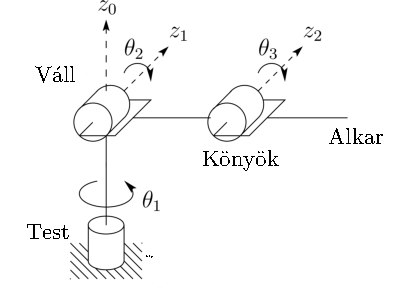
\includegraphics[width=0.3\linewidth]{./images/Elbow_manipulator}\hspace{1cm}
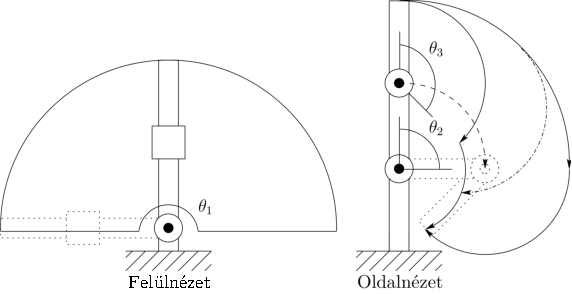
\includegraphics[width=0.5\linewidth]{./images/Elbow_workspace}
\caption{Az antropomorf robotkar felépítése és munkatere}
\end{figure}

Ez az egyik leggyakrabban használt robotkar, mivel szerkezetéből adódóan kiválóan alkalmas az emberi munkavégzés 
kiváltására. Munkatere gömb alakú, ezen belül viszonylag nagy mozgási szabadsággal rendelkezik.

\subsection{A gömbi robotkar (RRP)}
Az antropomorf manipulátor könyökét eltoló ízületre cserélve kapjuk a gömbi robotkart. Az elnevezés abból ered, hogy 
ekkor a három ízületi paraméter megegyezik a kéz egy olyan rendszer szerinti gömbi koordinátáival, melynek origója a 
hatástengelyek metszéspontjában van.
\begin{figure}[h]
\centering
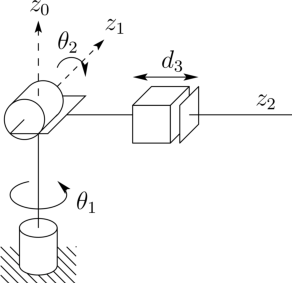
\includegraphics[width=0.35\linewidth]{./images/Spherical_manipulator}\hspace{1cm}
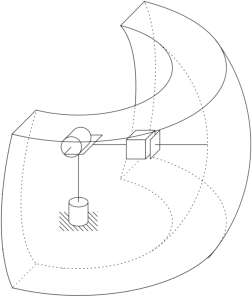
\includegraphics[width=0.35\linewidth]{./images/Spherical_workspace}
\caption{A gömbi robotkar felépítése és munkatere}
\end{figure}

\subsection{A hengeres robotkar (RPP)}
A hengeres robotkar első ízülete forgató, a második és a harmadik pedig eltoló. Ahogyan a neve is mutatja, az 
ízületi paraméterek megegyeznek a kéz hengerkoordinátáival, amennyiben az origót a manipulátor alapjának közepébe 
helyezzük.
\begin{figure}[h]
\centering
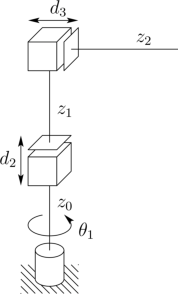
\includegraphics[width=0.25\linewidth]{./images/Cylindrical_manipulator}\hspace{1cm}
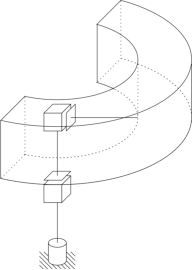
\includegraphics[width=0.35\linewidth]{./images/Cylindrical_workspace}
\caption{A hengeres robotkar felépítése és munkatere}
\end{figure}

\section{Direkt és inverz kinematika}
A direkt kinematikai feladat megoldásához szükségünk lesz egy jól meghatározott koordináta-rendszerre, amelyben meg 
tudjuk adni a kéz koordinátáit az ízületi paraméterek függvényében. Ezt úgy érjük el, hogy minden egyes szegmenshez 
mereven rögzítünk egy-egy koordináta-rendszert, azután pedig koordináta-transzformációkat hajtunk végre. 

Az $i$-edik szegmens koordináta-rendszerét jelölje $(o_i, x_i, y_i, z_i)$. Ebben a koordináta`=rendszerben az $i$-
edik szegmens pontjainak a koordinátái állandóak. A nulladik rendszert bázisrendszernek hívjuk, az $n$-ediket pedig 
a kéz koordináta-rendszerének.

\subsection{A Denavit-Hartenberg konvenció}
Olyan koordináta-rendszereket keresünk, amelyek kielégítik az alábbi feltételeket:

\begin{enumerate}[label=(\alph*)]
\item A $z_i$ tengely egybeesik az $i+1$-edik ízület hatástengelyével. \label{itm:zaxis}
\item Az $x_i$ tengely merőlegesen metszi a $z_{i-1}$ tengelyt. \label{itm:xaxis}
\end{enumerate}

\begin{figure}[h]
\centering
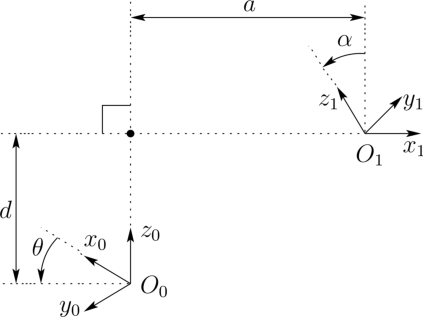
\includegraphics[width=0.5\linewidth]{./images/DH_convention}
\caption{A Denavit-Hartenberg konvenció}
\end{figure}

\begin{áll}
Mindig lehetséges így megválasztani a koordináta-rendszereket.
\end{áll}

\begin{proof}
A bázis koordináta-rendszerben csak a $z_0$ tengely van egyértelműen meghatározva, az első ízület 
hatástengelyeként. Az $o_0$ origó tetszőlegesen megválasztható ezen a tengelyen, illetve az $x_0$ tengely is 
tetszőleges, $o_0$ ponton átmenő, $z_0$-ra merőleges egyenes lehet. Ezek rögzítése után az $y_0$ tengely már 
egyértelműen meghatározott lesz.

Tegyük fel, hogy az első $i-1$ koordináta-rendszert már meghatároztuk a feltételeknek megfelelően. Ekkor 
\ref{itm:zaxis} szerint a $z_i$ tengely adott. Tudjuk továbbá, hogy az $x_i$ tengely merőlegesen metszi $z_i$-t, 
valamint \ref{itm:xaxis} alapján $z_{i-1}$-t is. Ebből kapjuk, hogy $x_i$ a $z_{i-1}$ és $z_i$ egyenesek normál 
transzverzálisa, ha $z_{i-1}$ és $z_i$ kitérő nem párhuzamos egyenesek, vagy a két egyenes metszéspontjában állított 
merőleges, ha $z_{i-1}$ és $z_i$ metsző, de nem egybeeső egyenesek. Abban az esetben, amikor $z_{i-1}$ és $z_i$ 
párhuzamosak vagy egybeesnek, az $x_i$ tengely tetszőleges rájuk merőleges egyenes lehet. Ilyenkor célszerű azt 
választani, amellyel a legegyszerűbb számolni. Ha $x_i$-t és $z_i$-t már meghatároztuk, akkor $o_i$-t a tengelyek 
metszeteként, $y_i$-t pedig a jobb-rendszer harmadik tagjaként kapjuk.
\end{proof}

\begin{figure}[h]
\centering
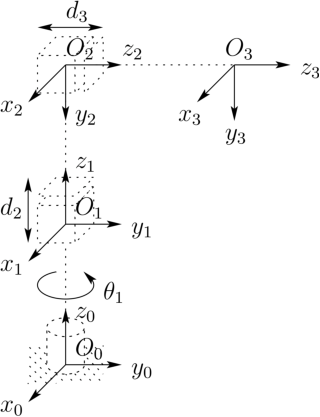
\includegraphics[width=0.35\linewidth]{./images/Cylindrical_frames}
\caption{A hengeres manipulátor koordináta-rendszerei}
\end{figure}

Tudjuk, hogy minden térbeli koordináta-rendszerek közötti irányítástartó transzformáció megadható hat adattal. Az 
eltolás leírható az eltolásvektor három koordinátájával, a forgatást pedig reprezentálhatjuk három Euler-szöggel 
vagy egy tisztán képzetes egységkvaternióval, amely szintén három adat. A pontos megadásra nem lesz szükségünk, 
ezért nem is részletezzük, de megtalálhatóak például \az+\autocite{spong_robot} jegyzetben.  Most megmutatjuk, hogy 
a Denavit-Hartenberg konvenció használatával négy paraméter is elegendő. Ennek az az oka, hogy ebben az esetben 
speciális helyzetű koordináta-rendszerek között hajtjuk végre a transzformációkat.

Hozzunk létre egy új, köztes koordináta-rendszert. Legyen $o'_i = x_i \cap z_{i-1}$, $x'_i = x_i$ és 
$z'_i = z_{i-1}$. Ekkor már $y'_i$ is adott. Legyen továbbá $d_i = |o'_i - o_{i-1}|$ illetve $a_i = |o_i - o'_i|$ az 
origók távolságai, valamint $\alpha_i = z'_i z_i \sphericalangle$ és $\theta_i = x_{i-1} x'_i \sphericalangle$ a 
tengelyek által bezárt szögek. Mivel $o'_i - o_{i-1} = d_i z_{i-1}$ és $o_i - o'_i = a_i x'_i$, így a 
$(d_i, a_i, \theta_i, \alpha_i)$ paraméterekkel leírható az $(o_i, x_i, y_i, z_i)$ koordináta-rendszer helyzete az 
$(o_{i-1}, x_{i-1}, y_{i-1}, z_{i-1})$ koordináta-rendszerben. Tehát ebben a speciális helyzetben a két rendszer 
viszonyának megadásához a szokásos hat paraméter helyett négy is elegendő. Most belátjuk, hogy ebből a négy adatból 
mindig csak egy fog változni az ízület mozgása során. Ezt nevezzük az adott ízület paraméterének.

\begin{figure}[ht]
\centering
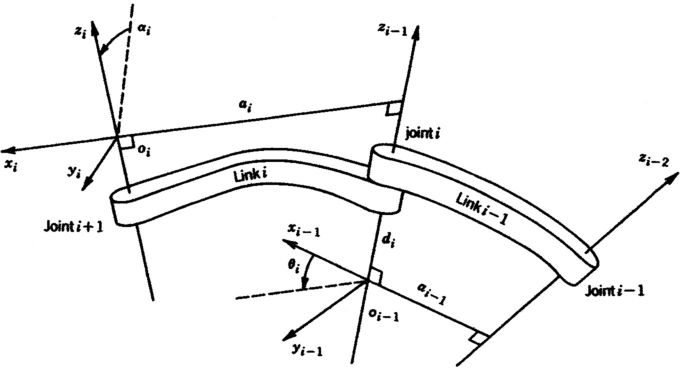
\includegraphics[width=0.9\linewidth]{./images/Link_frames}
\caption{Ízületi paraméterek és koordináta-rendszerek}
\end{figure}

\begin{áll}
Minden ízületre a négy paraméter $(d_i, a_i, \theta_i, \alpha_i)$ közül három konstans, és csak $\theta_i$ vagy 
$d_i$ változhat attól függően, hogy az $i$-edik ízület forgató vagy eltoló.
\end{áll}

\begin{proof}
Vegyük észre, hogy az $a_i$ és $\alpha_i$ paraméterek értékei nem változnak az ízület mozgásakor, mert azok csak a
$z_i$ és $z_{i-1}$ tengelyek helyzetétől, azaz csak a szegmens alaki tulajdonságaitól függenek. Forgató ízület 
esetében $d_i$ is állandó marad, mert nem történik eltolás, és így nem változik a tengelyek távolsága. Ekkor viszont 
$\theta_i$ pont az $i$-edik szegmens $z_{i-1}$ körüli elfordulását adja meg, azaz a forgató ízületek paramétere 
$\theta_i$ lesz. Hasonlóan, amikor az $i$-edik ízület eltoló, akkor $\theta_i$ lesz konstans, mert nem megy végbe 
forgatás, és így a tengelyek szöge állandó marad. Ebben az esetben $d_i$ fog változni, mégpedig az $i$-edik és az 
${i-1}$-edik ízület távolságának megfelelően, tehát az eltoló ízületek paramétere $d_i$.
\end{proof}

\subsection{A direkt kinematikai feladat}

Most vizsgáljuk meg, hogyan adható meg egy pont koordinátája egy másik ízület koordináta-rendszerében. Ehhez 
használjuk a pontok négydimenziós homogén koordinátáit, mivel így a lineáris transzformációk is könnyen kezelhetőek. 
Ekkor a direkt kinematikai feladat megoldásának számító transzformációt
\begin{equation}
T^{0}_{n} = \begin{bmatrix}
    R^{0}_{n} & o^{0}_{n} \\ 
    0 & 1
    \end{bmatrix} 
\end{equation} 
alakban keressük, ahol $R^{0}_{n} \in \mathbb{R}^{3 \times 3}$ a kéz rendszerének elfordulása a bázisrendszerhez 
képest, $o^{0}_{n} \in \mathbb{R}^3$ pedig a bázis origójából a kéz origójába mutató vektor.

Tekintsünk egy $(u_i, v_i, w_i, 1)^T$ pontot az $(o_i, x_i, y_i, z_i)$ koordináta-rendszerben. Ennek a pontnak az 
$(o'_i, x'_i, y'_i, z'_i)$ rendszer szerinti koordinátáit úgy kapjuk, hogy először eltoljuk az $x_i = x'_i$ tengely 
mentén $a_i$-vel, majd ugyanezen tengely mentén elforgatjuk $\alpha_i$ szöggel. Ezeknek a transzformációknak a 
szorzata a
\begin{equation}
T^{i'}_{i} =
\begin{bmatrix}
1 & 0 & 0 & 0 \\ 
0 & \cos \alpha_i & -\sin \alpha_i & 0 \\ 
0 & \sin \alpha_i & \cos \alpha_i & 0 \\ 
0 & 0 & 0 & 1
\end{bmatrix} 
\begin{bmatrix}
1 & 0 & 0 & a_i \\ 
0 & 1 & 0 & 0 \\ 
0 & 0 & 1 & 0 \\ 
0 & 0 & 0 & 1
\end{bmatrix} =
\begin{bmatrix}
1 & 0 & 0 & a_i \\ 
0 & \cos \alpha_i & -\sin \alpha_i & 0 \\ 
0 & \sin \alpha_i & \cos \alpha_i & 0 \\ 
0 & 0 & 0 & 1
\end{bmatrix} 
\end{equation}
mátrix. A köztes koordináta-rendszerből az $(o_{i-1}, x_{i-1}, y_{i-1}, z_{i-1})$ rendszerbe való áttéréshez végre 
kell még hajtanunk egy $d_i$-vel való eltolást és egy $\theta_i$ szögű forgatást a $z'_i = z_{i-1}$ tengely mentén. 
Ezt a transzformációt a
\begin{equation}
T^{i-1}_{i'} =
\begin{bmatrix}
\cos \theta_i & -\sin \theta_i & 0 & 0 \\ 
\sin \theta_i & \cos \theta_i & 0 & 0 \\ 
0 & 0 & 1 & 0 \\ 
0 & 0 & 0 & 1
\end{bmatrix} 
\begin{bmatrix}
1 & 0 & 0 & 0 \\ 
0 & 1 & 0 & 0 \\ 
0 & 0 & 1 & d_i \\ 
0 & 0 & 0 & 1
\end{bmatrix} =
\begin{bmatrix}
\cos \theta_i & -\sin \theta_i & 0 & 0 \\ 
\sin \theta_i & \cos \theta_i & 0 & 0 \\ 
0 & 0 & 1 & d_i \\ 
0 & 0 & 0 & 1
\end{bmatrix} 
\end{equation}
mátrix adja meg. Ezek alapján az $(o_i, x_i, y_i, z_i)$ rendszerből az $(o_{i-1}, x_{i-1}, y_{i-1}, z_{i-1})$ 
rendszerbe való áttérés mátrixa
\begin{equation}
\begin{aligned}
T^{i-1}_{i} &= T^{i-1}_{i'} T^{i'}_{i} = 
    \begin{bmatrix}
    R^{i-1}_{i} & o^{i-1}_{i} \\ 
    0 & 1
    \end{bmatrix} = \\
&= \begin{bmatrix}
    \cos \theta_i & -\sin \theta_i & 0 & 0 \\ 
    \sin \theta_i & \cos \theta_i & 0 & 0 \\ 
    0 & 0 & 1 & d_i \\ 
    0 & 0 & 0 & 1
    \end{bmatrix} 
    \begin{bmatrix}
    1 & 0 & 0 & a_i \\ 
    0 & \cos \alpha_i & -\sin \alpha_i & 0 \\ 
    0 & \sin \alpha_i & \cos \alpha_i & 0 \\ 
    0 & 0 & 0 & 1
    \end{bmatrix} = \\
&= \begin{bmatrix}
    \cos \theta_i  & -\cos \alpha_i \sin \theta_i & \sin \theta_i \sin \alpha_i & a_i \cos \theta_i \\ 
    \sin \theta_i & \cos \theta_i \cos \alpha_i & -\cos \theta_i \sin \alpha_i & a_i \sin \theta_i \\ 
    0 & \sin \alpha_i & \cos \alpha_i & d_i \\ 
    0 & 0 & 0 & 1
    \end{bmatrix}
\end{aligned}
\end{equation}
alakú. Tehát az $(u_i, v_i, w_i, 1)^T$ pont koordinátáit az $(o_{i-1}, x_{i-1}, y_{i-1}, z_{i-1})$ rendszerben az
\begin{equation}
\begin{bmatrix}
u_{i-1} \\ 
v_{i-1} \\ 
w_{i-1} \\ 
1
\end{bmatrix} =
\begin{bmatrix}
\cos \theta_i  & -\cos \alpha_i \sin \theta_i & \sin \theta_i \sin \alpha_i & a_i \cos \theta_i \\ 
\sin \theta_i & \cos \theta_i \cos \alpha_i & -\cos \theta_i \sin \alpha_i & a_i \sin \theta_i \\ 
0 & \sin \alpha_i & \cos \alpha_i & d_i \\ 
0 & 0 & 0 & 1
\end{bmatrix} 
\begin{bmatrix}
u_i \\ 
v_i \\ 
w_i \\ 
1
\end{bmatrix}
\end{equation}
összefüggés adja meg.

Legyenek a robot kezének koordinátái a hozzá tartozó $(o_n, x_n, y_n, z_n)$ rendszerben $(u_n, v_n, w_n, 1)^T$. 
Ekkor az előzőek alapján a direkt kinematikai feladat megoldása, azaz a kéz koordinátái az $(o_0, x_0, y_0, z_0)$ 
rendszerben
\begin{equation}
\begin{bmatrix}
u_0 \\ 
v_0 \\ 
w_0 \\ 
1
\end{bmatrix} =
T^{0}_{1} T^{1}_{2} \cdots T^{n-1}_{n}
\begin{bmatrix}
u_n \\ 
v_n \\ 
w_n \\ 
1
\end{bmatrix}
\end{equation}
ahol $T^{0}_{1}, T^{1}_{2}, \ldots, T^{n-1}_{n}$ az egyes ízületekhez tartozó, a fenti alakban előálló áttérési 
mátrixok. A $T^{0}_{n} = T^{0}_{1} T^{1}_{2} \cdots T^{n-1}_{n}$ mátrixból a kéz rendszerének elfordulása is könnyen 
leolvasható a fent említettek alapján.

\subsection{Az inverz kinematikai feladat}
A kéz adott helyzetét megvalósító ízületi paraméterek általános képlettel való meghatározása sokkal nehezebb a 
direkt feladat megoldásánál, mivel azt egy nemlineáris kifejezés adja meg. Habár konkrét robotkarok esetében 
geometriai okoskodással viszonylag könnyen kiszámíthatóak ezek a paraméterek, általában több lehetséges megoldás is 
tartozik a kéz egy kívánt helyzetéhez, és gyakran nem egyértelmű, hogy melyiket érdemes választani. 

Ez a probléma azonban sokkal elegánsabban megoldható a sebességkinematika és az útkeresés segítségével, amely 
feladatokat egy robotkar programozásához egyébként is meg kell oldanunk. Ekkor ugyanis nem csupán egy kívánt 
pozíciót és orientációt szabunk meg a kéznek, hanem egy teljes útvonalat, és annak minden pontjára adott lineáris és 
szögsebességeket is előírunk. Ezáltal egy egyértelmű megoldást kapunk a kéz tetszőleges helyzetbe történő 
elmozgatására.

\chapter{Sebességkinematika}
Az előzőekben azt vizsgáltuk, hogy milyen kapcsolat van az ízületi paraméterek és a robotkar pozíciója között. Ennek 
segítségével megtudhatjuk, hogy adott paraméterek esetén hol van éppen a kar, vagy hogy az ízületek milyen állásánál 
kerül a kar a kívánt pozícióba. Ez azonban önmagában még nem elég ahhoz, hogy egy robotot vezérelni tudjunk. Nem 
mindegy ugyanis, hogy milyen sebességgel kerül a robot a kívánt helyzetbe. Ha túl gyorsan mozog, kárt tehet a 
környezetében vagy akár saját magában is. Ha pedig túl lassan, akkor minden mozgás szükségtelenül sok időt vesz 
igénybe. A pontos sebességekre akkor is szükségük van, amikor emberi mozgásokat szeretnénk élethűen utánozni. 
Ilyenkor fontos, hogy a kar mozgása életszerű, folytonos sebességgel történjen. Ahogy a bevezetőben is szóba került, 
ez segít abban, hogy az animált karakterek mozgása valósághű legyen.

A korábbiakhoz hasonlóan most is kétféle problémát különböztetünk meg: a direkt és az inverz sebességkinematikai 
feladatot. Az előbbinél adottak az ízületek sebességei, azaz a paraméterek deriváltjai, és keressük a kar eredő 
sebességét. Az utóbbinál adott sebességgel szeretnénk mozgatni a robotkart, és keressük az ezt megvalósító 
paraméter-deriváltakat. A direkt kinematikai egyenletek meghatároznak egy leképezést az ízületi paraméterek és a kar 
pozíciója között. A sebességkinematikai problémák megoldásához szükségünk lesz ennek a deriváltjára, azaz a 
Jacobi-mátrixra. Ez az egyik legfontosabb mennyiség a robotgeometriában, szinte minden területen felmerül: az 
útvonalkeresés és -követésben, a szinguláris pozíciók meghatározásában, a mozgás dinamikai egyenleteinek 
levezetésében, illetve a robotkarra ható erő és nyomaték kiszámításában.

Mielőtt rátérnénk ezekre a problémákra, és kiszámítanánk a Jacobi-mátrixot, tekintsük meg, hogyan 
jellemezhető egy test lineáris- illetve szögsebessége, valamint hogyan tudjuk ezeket könnyedén kiszámítani. Ehhez 
megismerkedünk a ferdén szimmetrikus mátrixokkal, és megvizsgáljuk a forgatási mátrixokhoz és a szögsebességhez való 
viszonyukat. Ezek ismeretében a Jacobi-mátrix már könnyen meghatározható.

\section{Ferdén szimmetrikus mátrixok és a szögsebesség}
Tekintsünk egy olyan esetet, amikor egy merev test egy rögzített tengely körül forog. Ekkor a test egyes pontjai 
olyan körpályákon fognak mozogni, amelyek középpontjai a tengelyre esnek. A mozgás során adott idő alatt minden 
egyes pont ugyanakkora szöggel fordul el a pálya középpontja körül. A $t$ idő alatti szögelfordulást jelölje 
$\theta(t)$. Legyen $k$ egy forgástengellyel párhuzamos egységvektor. Ekkor a szögsebesség szabad vektora
\begin{equation}
\omega = \dot{\theta}k
\end{equation}
ahol $\dot{\theta}$ az idő szerinti deriváltja $\theta$-nak. Itt a szabad vektor azt jelenti, hogy $\omega$ egy 
irányított szakasz, azaz csak a nagysága és az iránya adott, és így tetszőleges rendszer megfelelő helyvektorával 
reprezentálható. A képlet azt mutatja, hogy a szögsebesség egy olyan, a forgás tengelyébe eső vektor, melynek 
nagysága az elfordulás megváltozásával arányos, az iránya pedig a forgásirányból a jobbkéz-szabály alapján kapható.

Tudjuk, hogy adott szögsebesség mellett a test egy pontjának lineáris sebessége
\begin{equation}
v = \omega \times r
\end{equation}
ahol $r$ az origóból a pontba mutató vektor.

\begin{figure}[h]
\centering
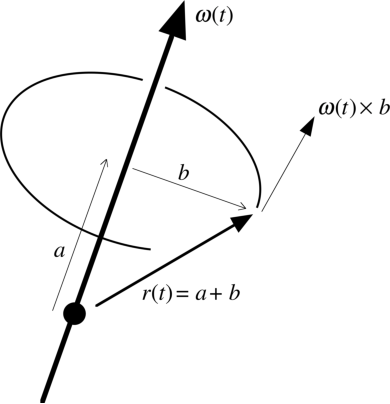
\includegraphics[width=0.5\linewidth]{./images/Angular_velocity}
\caption{A szögsebesség és a lineáris sebesség}
\end{figure}

Az előzőekhez hasonlóan a testek helyzetét most is a hozzájuk rendelt koordináta-rendszer helyzetével fogjuk 
leírni. Mivel a test minden pontjában ugyanakkora a szögsebesség, és a testhez mereven rögzített koordináta-rendszer 
minden ponthoz képest fix, ezért a szögsebesség magának a koordináta-rendszernek a jellemzője.

A szögsebesség további vizsgálatához szükségünk lesz a ferdén szimmetrikus mátrixokra és azok tulajdonságaira. 
Ezek segítségével egyszerűen ki tudjuk számítani forgatási mátrixok deriváltjait, valamint meg tudjuk határozni a 
hozzájuk tartozó szögsebességet. Ezáltal egy könnyen használható, minden dimenzióban általánosan alkalmazható 
modellhez jutunk.

\subsection{A ferdén szimmetrikus mátrixok}
Ahhoz, hogy meghatározzuk a koordináta-rendszerek egymáshoz viszonyított sebességei közötti transzformációkat, ki 
kell tudnunk számítani egy forgatási mátrix deriváltját. Ferdén szimmetrikus mátrixok használatával ezen számítások 
jelentősen leegyszerűsíthetőek.
\begin{defi}
Egy $n \times n$-es $S$ mátrixot pontosan akkor nevezünk ferdén szimmetrikusnak, ha
\begin{equation}
S^T + S = 0
\end{equation}
ahol $0$ a nullmátrixot jelöli.
\end{defi}
Az ilyen mátrixok halmazát $\mathfrak{so}(n)$-nel jelöljük. Ez a jelölés onnan származik, hogy az $SO(n)$ csoport 
Lie-algebrája $\mathfrak{so}(n)$, amelyet épp a ferdén szimmetrikus mátrixok alkotnak. A definícióból következik, 
hogy minden 
$S \in \mathfrak{so}(n)$-re 
\begin{equation}
s_{ij} = \begin{dcases*}
    -s_{ji} & ha $i \neq j$\\
    0 & ha $i = j$
    \end{dcases*}
\end{equation}
Tehát miden $3 \times 3$-as ferdén szimmetrikus mátrixnak csak $3$ független eleme van, és így a következő alakban 
írható fel
\begin{equation}
S = \begin{bmatrix}
    0 & -s_3 & s_2 \\ 
    s_3 & 0 & -s_1 \\ 
    -s_2 & s_1 & 0
    \end{bmatrix} 
\end{equation}
Vegyünk egy $a = (a_x, a_y, a_z)^T$ vektort. Ekkor hozzárendelhető egy
\begin{equation} \label{eq:generatedskew}
S(a) = \begin{bmatrix}
    0 & -a_z & a_y \\ 
    a_z & 0 & -a_x \\ 
    -a_y & a_x & 0
    \end{bmatrix} 
\end{equation}
mátrix, melyet az $a$ által generált ferdén szimmetrikus mátrixnak nevezünk.

\begin{pl}
Jelölje a szokott módon $i, j$ és $k$ a koordináta-rendszer három bázisvektorát. Nézzük meg az ezek által generált 
ferdén szimmetrikus mátrixokat, mivel ezeknek a későbbiekben még hasznát fogjuk venni. Az előzőek szerint 
$S(i), S(j)$ és $S(k)$
\begin{equation}
S(i) = \begin{bmatrix}
    0 & 0 & 0 \\ 
    0 & 0 & -1 \\ 
    0 & 1 & 0
    \end{bmatrix}, \quad
S(j) = \begin{bmatrix}
    0 & 0 & 1 \\ 
    0 & 0 & 0 \\ 
    -1 & 0 & 0
    \end{bmatrix}, \quad
S(k) = \begin{bmatrix}
    0 & -1 & 0 \\ 
    1 & 0 & 0 \\ 
    0 & 0 & 0
    \end{bmatrix} 
\end{equation}
alakúak.
\end{pl}

Most vizsgáljuk meg a ferdén szimmetrikus mátrixok néhány olyan tulajdonságát, amelyekre a továbbiakban gyakran 
fogunk hivatkozni, és amelyekre szükségünk lesz például a Jacobi-mátrix meghatározásánál is.

\begin{enumerate}[label=\arabic*.]
\item Az $S$ operátor lineáris, azaz
    \begin{equation}
    S(\alpha a + \beta b) = \alpha S(a) + \beta S(b)
    \end{equation}
    bármely $a, b \in \mathbb{R}^3$ vektorra és tetszőleges $\alpha, \beta \in \mathbb{R}$ skalárra.
\item Minden $a, p \in \mathbb{R}^3$ vektorra
    \begin{equation} \label{eq:skewcross}
    S(a)p = a \times p
    \end{equation}
    Ez az összefüggés a két oldal kiszámításával egyszerűen ellenőrizhető.
\item Minden $R \in SO(3)$ forgatásra és $a \in \mathbb{R}^3$ vektorra
    \begin{equation} \label{eq:skewtransf}
    RS(a)R^T = S(Ra)
    \end{equation}
    Ezen állítás bizonyításához szükségünk van a forgatómátrixok egyik tulajdonságára, mely szerint minden 
    $R \in SO(3)$ forgatásra és $a, b \in \mathbb{R}^3$ vektorra
    \begin{equation} \label{eq:rotdistrib}
    R(a \times b) = Ra \times Rb
    \end{equation}
    azaz a forgatás disztributív a vektorszorzásra nézve. Ez az adott műveletek geometriai jelentéséből 
    következik. Tetszőleges $b \in \mathbb{R}^3$ vektorra \az+\eqref{eq:skewcross} egyenletből
    \begin{equation}
    RS(a)R^Tb = R(a \times R^Tb)
    \end{equation}
    adódik. Erre \az+\eqref{eq:rotdistrib} összefüggést alkalmazva, és a szorzást elvégezve
    \begin{equation}
    R(a \times R^Tb) = (Ra) \times (RR^Tb) = (Ra) \times b
    \end{equation}
    jön ki. Ekkor \eqref{eq:skewcross} ismételt alkalmazásával
    \begin{equation}
    (Ra) \times b = S(Ra)b
    \end{equation}
    kapható, azaz beláttuk, hogy
    \begin{equation}
    RS(a)R^Tb = S(Ra)b
    \end{equation}
    minden $b$ vektorra.
\end{enumerate}

\subsection{A forgatási mátrixok deriválása}
Tegyük fel, hogy az $R$ forgatási mátrix a $\theta$ változó függvénye, azaz $R = R(\theta) \in SO(3)$ minden 
$\theta \in \mathbb{R}$-re. Ilyen például, amikor egy rögzített tengely körül forgatunk $\theta$ szöggel, de 
természetesen az alábbiak ennél általánosabb esetben is érvényesek. Mivel $R$ minden $\theta$ paraméterre 
ortogonális, ezért
\begin{equation}
R(\theta)R(\theta)^T = I
\end{equation}
adódik. Mindkét oldalt $\theta$ szerint deriválva, a szorzat-szabályt felhasználva, és figyelembe véve, hogy a 
konstans mátrix deriváltja $0$, azt kapjuk, hogy
\begin{equation} \label{eq:rotderiv}
\diff{R}{\theta}R(\theta)^T + R(\theta)\diff{R^T}{\theta} = 0
\end{equation}
Vezessük be az első tagra az
\begin{equation} \label{eq:skewdef}
S := \diff{R}{\theta}R(\theta)^T
\end{equation}
jelölést. Mivel $S$ transzponáltja
\begin{equation}
S^T = \left(\diff{R}{\theta}R(\theta)^T\right)^T = R(\theta)\diff{R^T}{\theta}
\end{equation}
Ezért \az+\eqref{eq:rotderiv} egyenlet
\begin{equation}
S + S^T = 0
\end{equation}
alakra hozható, vagyis az $S$ mátrix definíció alapján ferdén szimmetrikus. Ha \az+\eqref{eq:skewdef} egyenletet 
$R$-rel jobbról megszorozzuk, és felhasználjuk, hogy a jobb oldalon $R^TR = I$ teljesül, akkor azt kapjuk, hogy
\begin{equation} \label{eq:rotskewderiv}
\diff{R}{\theta} = SR(\theta)
\end{equation}
ami a forgatási mátrixok deriválási szabálya. Ezt az összefüggést a későbbiekben gyakran fogjuk alkalmazni. Eszerint 
egy $R$ forgatási mátrix deriváltjának kiszámítása ekvivalens egy $S$ ferdén szimmetrikus mátrixszal való 
mátrixszorzással.

\begin{pl}
Vegyük most azt a példát, amire a bevezetőben utaltunk. Legyen $R = R_{x, \theta}$ az $x$ tengely körüli, $\theta$ 
szögű forgatás mátrixa. Mivel
\begin{equation}
R_{x, \theta} = 
    \begin{bmatrix}
    1 & 0 & 0 \\ 
    0 & \cos \theta & -\sin \theta \\ 
    0 & \sin \theta & \cos \theta
    \end{bmatrix}
\quad\textrm{ és }\quad 
\diff{R}{\theta} = 
    \begin{bmatrix}
    0 & 0 & 0 \\ 
    0 & -\sin \theta & -\cos \theta \\ 
    0 & \cos \theta & -\sin \theta
    \end{bmatrix} 
\end{equation}
ezért a transzponálttal való mátrixszorzást elvégezve
\begin{equation}
\begin{aligned}
\diff{R}{\theta}R^T &= 
    \begin{bmatrix}
    0 & 0 & 0 \\ 
    0 & -\sin \theta & -\cos \theta \\ 
    0 & \cos \theta & -\sin \theta
    \end{bmatrix} 
    \begin{bmatrix}
    1 & 0 & 0 \\ 
    0 & \cos \theta & \sin \theta \\ 
    0 & -\sin \theta & \cos \theta
    \end{bmatrix} = \\
&= \begin{bmatrix}
0 & 0 & 0 \\ 
0 & 0 & -1 \\ 
0 & 1 & 0
\end{bmatrix} 
= S(i)
\end{aligned}
\end{equation}
adódik. Tehát azt az összefüggést kaptuk, mely szerint 
\begin{equation}
\diff{R_{x, \theta}}{\theta} = S(i)R_{x, \theta}
\end{equation}
ahol $i = (1, 0, 0)^T$ az egyik bázisvektor. Hasonló számolással bizonyítható, hogy
\begin{equation}
\diff{R_{y, \theta}}{\theta} = S(j)R_{y, \theta} \quad\textrm{ és }\quad \diff{R_{z, \theta}}{\theta} = S(k)R_{z, 
\theta}
\end{equation}
a $j = (0, 1, 0)^T$ és $k = (0, 0, 1)^T$ bázisvektorokra. Továbbá könnyen belátható, hogy tetszőleges $g$ tengelyre, 
melynek egységvektora $e$, az $R_{g, \theta}$ forgatás deriváltja
\begin{equation}
\diff{R_{g, \theta}}{\theta} = S(e)R_{g, \theta}
\end{equation}
\end{pl}

\section{Az eredő lineáris és szögsebesség}
Tekintsük most azt az általánosabb esetet, amikor a forgástengely tetszőleges, origón átmenő, akár mozgó egyenes is 
lehet. Tegyük fel, hogy az $R$ forgatási mátrix függ az időtől, azaz $R = R(t) \in SO(3)$ minden 
$t \in \mathbb{R}$-re. Az előzőekben $R$ paramétere ugyan a $\theta$ szög volt, de a formális számolások miatt ezek 
ugyanazt eredményezik, csupán a szemléletes jelentésük különböző. Ekkor az $R(t)$ mátrix idő szerinti deriváltja, 
feltéve, hogy $R(t)$ folytonosan differenciálható $t$ szerint, \az+\eqref{eq:rotskewderiv} képlet alapján
\begin{equation}
\dot{R}(t) = S(t)R(t)
\end{equation}
alakú, ahol $S(t)$ egy ferdén szimmetrikus mátrix. Ekkor $S(t)$ \az+\eqref{eq:generatedskew} egyenlet alapján a 
megfelelő komponensek leolvasásával $S(\omega(t))$ alakban reprezentálható egy $\omega(t)$ vektor segítségével. 
Belátható, hogy ez a vektor a forgó rendszer szögsebessége a $t$ időpillanatban a bázisrendszerhez viszonyítva. Így 
$R(t)$ idő szerinti deriváltja
\begin{equation} \label{eq:angderiv}
\dot{R}(t) = S(\omega(t))R(t)
\end{equation}
ahol $\omega(t)$ a szögsebesség.

\Az+\eqref{eq:angderiv} egyenlet a szögsebesség és a forgatási mátrix deriváltja közötti kapcsolatot adja meg. Ez 
alapján, ha az $(o_1, x_1, y_1, z_1)$ rendszer $(o_0, x_0, y_0, z_0)$ rendszerhez viszonyított pillanatnyi 
orientációját $R^{0}_{1}$ határozza meg, akkor az $\omega^{0}_{1}$ szögsebesség $R^{0}_{1}$ deriváltjától függ a 
fentiek szerint.

\begin{pl}
Az előző példát továbbgondolva legyen $R(t) = R_{x, \theta(t)}$. Ekkor a láncszabályt alkalmazva
\begin{equation}
\dot{R} = \diff{R}{t} = \diff{R}{\theta} \diff{\theta}{t}
\end{equation}
adódik, melyből az előző példa eredménye alapján
\begin{equation}
\diff{R}{\theta} \diff{\theta}{t} = S(i)R(t)\dot{\theta} = S(\omega(t))R(t)
\end{equation}
kapható, ahol $S$ linearitását felhasználva $\omega = i\dot{\theta}$ a szögsebesség, $i = (1, 0, 0)^T$ pedig az 
egyik bázisvektor. Hasonló összefüggés igaz tetszőleges tengelyű forgatásra is.
\end{pl}

\subsection{Szögsebességek összege}
A robotkarok vizsgálata során a Denavit-Hartenberg konvenció használatából adódóan több, egymáshoz képest forgó 
koordináta-rendszer eredő szögsebességére vagyunk kíváncsiak. Ennek kiszámításához most meghatározunk egy képletet 
két mozgó rendszer, $(o_1, x_1, y_1, z_1)$ és $(o_2, x_2, y_2, z_2)$ szögsebességeinek összegére, az 
$(o_0, x_0, y_0, z_0)$ rögzített koordináta`=rendszerhez viszonyítva.

Tegyük fel, hogy a három rendszernek közös az origója. Ez nem jelent megkötést, hiszen a szögsebesség invariáns az 
eltolásra nézve. Legyenek $R^{0}_{1}(t)$ és $R^{1}_{2}(t)$ az $(o_1, x_1, y_1, z_1)$ és $(o_2, x_2, y_2, z_2)$ 
koordináta-rendszerek relatív orientációját megadó, időtől függő forgatási mátrixok. Ekkor lineáris algebrából 
tudjuk, hogy
\begin{equation}
R^{0}_{2}(t) = R^{0}_{1}(t) R^{1}_{2}(t)
\end{equation}
Ha mindkét oldalát deriváljuk az idő szerint, akkor azt kapjuk, hogy
\begin{equation} \label{eq:rotprodderiv}
\dot{R^{0}_{2}} = \dot{R^{0}_{1}} R^{1}_{2} + R^{0}_{1} \dot{R^{1}_{2}}
\end{equation}
\Az+\eqref{eq:angderiv} egyenlet értelmében $\dot{R^{0}_{2}}$ felírható
\begin{equation}
\dot{R^{0}_{2}} = S(\omega^{0}_{0,2}) R^{0}_{2}
\end{equation}
alakban. Ebben a kifejezésben $\omega^{0}_{0,2}$ az $(o_2, x_2, y_2, z_2)$ rendszerre ható eredő szögsebességet 
jelöli. Ez az $R^{0}_{1}$ és az $R^{1}_{2}$ mátrixok együttes forgatásából adódik.

Most vizsgáljuk meg \az+\eqref{eq:rotprodderiv} egyenlet jobb oldalát. Az első tagra \az+\eqref{eq:angderiv} képlet 
felhasználásával 
\begin{equation}
\dot{R^{0}_{1}} R^{1}_{2} = S(\omega^{0}_{0,1}) R^{0}_{1} R^{1}_{2} = S(\omega^{0}_{0,1}) R^{0}_{2}
\end{equation}
adódik. A jobb oldal második tagjára \az+\eqref{eq:angderiv} egyenlet újbóli felhasználásával azt kapjuk, hogy
\begin{equation}
R^{0}_{1} \dot{R^{1}_{2}} = R^{0}_{1} S(\omega^{1}_{1,2}) R^{1}_{2}
\end{equation}
Ezt az $I= (R^{0}_{1})^T R^{0}_{1}$ taggal bővítve
\begin{equation}
R^{0}_{1} S(\omega^{1}_{1,2}) R^{1}_{2} = R^{0}_{1} S(\omega^{1}_{1,2}) (R^{0}_{1})^T R^{0}_{1} R^{1}_{2}
\end{equation}
adódik, melyből \az+\eqref{eq:skewtransf} egyenlet alapján
\begin{equation}
R^{0}_{1} S(\omega^{1}_{1,2}) (R^{0}_{1})^T R^{0}_{1} R^{1}_{2}
    = S(R^{0}_{1}\omega^{1}_{1,2}) R^{0}_{1} R^{1}_{2}
    = S(R^{0}_{1}\omega^{1}_{1,2}) R^{0}_{2}
\end{equation}
következik. Tehát azt kaptuk, hogy
\begin{equation}
R^{0}_{1} \dot{R^{1}_{2}} = S(R^{0}_{1}\omega^{1}_{1,2}) R^{0}_{2}
\end{equation}
Ebben az egyenletben $\omega^{1}_{1,2}$ az $(o_2, x_2, y_2, z_2)$ rendszernek az $R^{1}_{2}$ megváltozásához tartozó 
szögsebességét jelöli, az $(o_1, x_1, y_1, z_1)$ koordináta-rendszerben felírva. Az $R^{0}_{1}\omega^{1}_{1,2}$ 
szorzat ezt a szögsebességet az $(o_0, x_0, y_0, z_0)$ rendszerhez viszonyítva fejezi ki, azaz 
$R^{0}_{1}\omega^{1}_{1,2}$ az $\omega_{1,2}$ szabad vektor koordinátáit adja meg a $0$-dik rendszerben.

\Az+\eqref{eq:rotprodderiv} egyenlet két oldalán szereplő tagokra kapott összefüggések alapján az
\begin{equation}
S(\omega^{0}_{2})R^{0}_{2} = \left(S(\omega^{0}_{0,1}) + S(R^{0}_{1}\omega^{1}_{1,2})\right) R^{0}_{2}
\end{equation}
összefüggés adódik. Felhasználva az $S$ mátrix linearitását, azt kapjuk, hogy
\begin{equation}
\omega^{0}_{2} = \omega^{0}_{0,1} + R^{0}_{1}\omega^{1}_{1,2}
\end{equation}
Ezzel beláttuk azt az állítást, mely szerint a szögsebesség-vektorok összeadhatóak, ha ugyanabban a 
koordináta`=rendszerben, jelen esetben $(o_0, x_0, y_0, z_0)$-ban vannak felírva.

A fenti érvelés tetszőleges számú koordináta-rendszerre érvényes marad. Tegyük fel, hogy ismerjük az
\begin{equation}
R^{0}_{n} = R^{0}_{1}R^{1}_{2} \cdots R^{n-1}_{n}
\end{equation}
forgatási mátrixokat. A fenti bizonyításhoz hasonlóan igazolható, hogy ekkor
\begin{equation}
\dot{R^{0}_{n}} = S(\omega^{0}_{0,n}) R^{0}_{n}
\end{equation}
ahol
\begin{equation} \label{eq:angularsum}
\begin{aligned}
\omega^{0}_{0,n} &= \omega^{0}_{0,1} + R^{0}_{1}\omega^{1}_{1,2} + R^{0}_{2}\omega^{2}_{2,3} + \cdots +
    R^{0}_{n-1}\omega^{n-1}_{n-1,n} = \\ 
&= \omega^{0}_{0,1} + \omega^{0}_{1,2} + \omega^{0}_{2,3} + \cdots + \omega^{0}_{n-1,n}
\end{aligned}
\end{equation}

\subsection{Egy pont lineáris sebessége}
Tekintsünk egy $(o_0, x_0, y_0, z_0)$ rendszert, és egy hozzá képest forgómozgást végző $(o_1, x_1, y_1, z_1)$ 
rendszert, melyeknek közös az origója. Tegyük fel, hogy a $p$ pont mereven rögzítve van a mozgó rendszerhez. Most 
ennek a pontnak a lineáris sebességét fogjuk megvizsgálni. A $p$ koordinátáit az $(o_0, x_0, y_0, z_0)$ rendszerben
\begin{equation}
p^0(t) = R^{0}_{1}(t)p^1
\end{equation}
alakban kapjuk meg, ahol $p^i$ az $i$-edik rendszerben felírt koordinátákat jelöli. Ebből a szorzat deriválási 
szabálya alapján
\begin{equation}
\dot{p}^0 = \dot{R}^{0}_{1}p^1 + R^{0}_{1}\dot{p}^1
\end{equation}
adódik. Innen \az+\eqref{eq:angderiv} egyenlet alkalmazásával, valamint felhasználva, hogy $p$ koordinátái az 
$(o_1, x_1, y_1, z_1)$ rendszerben nem változnak, azt kapjuk, hogy
\begin{equation}
\dot{R}^{0}_{1}p^1 + R^{0}_{1}\dot{p}^1 = S(\omega^0)R^{0}_{1}p^1
\end{equation}
Végül a ferdén szimmetrikus mátrixok \eqref{eq:skewcross} tulajdonsága alapján
\begin{equation}
S(\omega^0)R^{0}_{1}p^1 = S(\omega^0)p^0 = \omega^0 \times p^0
\end{equation}
amely a már ismert kifejezés a sebesség kiszámítására.

Természetesen a két koordináta-rendszer mozgása ennél általánosabb is lehet, hiszen az $o_0$ és $o_1$ pontok 
távolsága is változhat. Ennek megfelelően jelölje $o^{0}_{1}(t)$ a bázisrendszer origójából az 
$(o_1, x_1, y_1, z_1)$ rendszer origójába mutató vektort. Ekkor a $p$ pont koordinátáit megadó transzformáció
\begin{equation}
p^0(t) = R^{0}_{1}(t)p^1 + o^{0}_{1}(t)
\end{equation}
alakú. Ezt a kifejezést a szorzat-szabály alapján deriválva kapjuk, hogy
\begin{equation}
\begin{aligned}
\dot{p}^0 &= \dot{R}p^1 + \dot{o} = \\
    &= S(\omega)Rp^1 + \dot{o}
\end{aligned}
\end{equation}
Ebből \az+\eqref{eq:skewcross} tulajdonság felhasználásával, valamint az $r = R^{0}_{1}p^1$ és $v = \dot{o}_1$ 
jelölések bevezetésével
\begin{equation}
S(\omega)Rp^1 + \dot{o} = \omega \times r + v
\end{equation}
adódik. Amennyiben a $p$ pont az $(o_1, x_1, y_1, z_1)$ rendszerhez képest is elmozdul, akkor $v$-hez még 
hozzá kell adnunk az $R\dot{p}^1$ tagot, amely a $p^1$ koordináták megváltozásának sebességét fejezi ki az
$(o_0, x_0, y_0, z_0)$ rendszerhez képest.

\section{A Jacobi-mátrix kiszámítása}
Az előzőekben kiszámoltuk a koordináta-rendszerek mozgásából adódó lineáris és szögsebességeket. Most ezen 
eredményeket felhasználva meghatározzuk a robotkar Jacobi-mátrixát, amellyel a direkt sebességkinematikai feladat 
már könnyen megoldható.

Tekintsünk egy $n$ ízületű robotkart, melynek ízületi paraméterei $q_1, \ldots, q_n$, ahol $q_i = d_i$, ha az ízület 
eltoló, és $q_i = \theta_i$, ha forgató. Jelölje
\begin{equation}
T^{0}_{n}(q) = \begin{bmatrix}
    R^{0}_{n}(q) & o^{0}_{n}(q) \\ 
    0 & 1
    \end{bmatrix} 
\end{equation}
a kéz koordináta-rendszeréből a bázisrendszerbe képező transzformációt, ahol $q = (q_1, \ldots, q_n)^T$ a 
paraméterek vektora. A robot mozgása során a $q_i$ változók az idő függvényei lesznek, de ekkor $R^{0}_{n}$ és 
$o^{0}_{n}$ is a $t$ paramétertől fognak függeni. Ebben a szakaszban megvizsgáljuk a kéz lineáris és 
szögsebességének a kapcsolatát az ízületi sebességek $\dot{q}(t)$ vektorával. \Az+\eqref{eq:angderiv} egyenlet 
alapján
\begin{equation}
S(\omega^{0}_{n}) = \dot{R^{0}_{n}}(R^{0}_{n})^T
\end{equation}
ahol $\omega^{0}_{n}$ a kéz szögsebesség-vektora. Vezessük be a kéz lineáris sebességére a 
$v^{0}_{n} = \dot{o}^{0}_{n}$ jelölést. Ekkor a direkt sebességkinematikai feladat értelmében olyan $J_v$ és 
$J_\omega$ $3 \times n$-es mátrixokat keresünk, melyek kielégítik a
\begin{equation}
\begin{aligned}
v^{0}_{n} &= J_v \dot{q} \\
\omega^{0}_{n} &= J_\omega \dot{q}
\end{aligned}
\end{equation}
egyenleteket. Ezt a két összefüggést egy közös képlettel is 
felírhatjuk
\begin{equation} \label{eq:jacobidef}
\xi = J\dot{q}
\end{equation}
alakban, ahol 
\begin{equation} 
\xi = \begin{bmatrix}
    v^{0}_{n} \\ 
    \omega^{0}_{n}
\end{bmatrix}
\quad\textrm{ és }\quad 
J = \begin{bmatrix}
    J_v \\ 
    J_\omega
\end{bmatrix}
\end{equation}
Itt fontos megjegyezni, hogy habár a $\xi$ vektor sebességet jelöl, mégsem egy helyváltozó idő szerinti deriváltja, 
mert a benne szereplő szögsebesség egy származtatott mennyiség. A $J$ mátrixot a robotkar Jacobi-mátrixának 
nevezzük. Ez egy $6 \times n$-es mátrix, ahol $n$ az ízületek száma. Vizsgáljuk meg jobban ezt a mátrixot, hogy egy 
könnyen kiszámítható képletet tudjunk adni rá.

\subsection{A kéz szögsebessége}
Az előző szakaszban már foglalkoztunk az eredő szögsebességgel, és \az+\eqref{eq:angularsum} összefüggés által azt 
kaptuk, hogy a szögsebességek összeadhatóak szabad vektorokként, feltéve, hogy azonos koordináta-rendszerben vannak 
felírva. Ez azt jelenti, hogy úgy tudjuk meghatározni a kéz szögsebességét a bázisrendszerhez képest, hogy 
meghatározzuk az egyes ízületek szögsebességét a bázisrendszerben felírva, majd összeadjuk őket. Mivel a robotkar 
ízületei forgatók és eltolók is lehetnek, vizsgáljuk meg a kéz szögsebességét mindkét esetben.

Ha az $i$-edik ízület forgató, akkor a $q_i$ ízületi paraméter $\theta_i$-vel egyezik meg, a forgatás tengelye pedig 
$z_{i-1}$. A korábbiakhoz hasonlóan jelölje $\omega^{i-1}_{i}$ az $i$-edik szegmens szögsebességét, amely az 
$i$-edik ízület mozgásából adódik, az $(o_{i-1}, x_{i-1}, y_{i-1}, z_{i-1})$ rendszerben felírva. Ez a szögsebesség 
az $i-1$-edik rendszerben kifejezhető
\begin{equation}
\omega^{i-1}_{i} = \dot{q}_i z^{i-1}_{i-1} = \dot{q}_i k
\end{equation}
alakban, ahol $z^{i-1}_{i-1} = k$ az $i-1$-edik rendszer $(0, 0, 1)^T$ koordinátájú bázisvektora.

Abban az esetben, amikor az $i$-edik ízület eltoló, az $i$-edik rendszer mozgása az $i-1$-edikhez képest egy 
eltolás. Mivel nem történik forgatás, így a szögsebességre
\begin{equation}
\omega^{i-1}_{i} = 0
\end{equation}
adódik. Ezért eltoló ízület esetében a kéz szögsebessége nem függ $q_i$-től, amely most $d_i$-vel egyenlő.

Az imént kapott összefüggéseket beírva \az+\eqref{eq:angularsum} egyenletbe, a kéz eredő szögsebessége a bázis 
koordináta-rendszerben
\begin{equation}
\omega^{0}_{n} = \delta_1\dot{q}_1 k + \delta_2\dot{q}_2 R^{0}_{1}k + \cdots + \delta_n\dot{q}_n R^{0}_{n-1}k
\end{equation}
alakú lesz, ahol $\delta_i$ értéke $1$, ha az $i$-edik ízület forgató, illetve $0$, ha az ízület eltoló. Ha 
felhasználjuk az
\begin{equation}
z^{0}_{i-1} = R^{0}_{i-1}k \qquad i = 1, \ldots, n
\end{equation}
összefüggést, ahol természetesen $z^{0}_{0} = k = (0, 0, 1)^T$, akkor a fenti egyenlet az
\begin{equation}
\omega^{0}_{n} = \sum^{n}_{i=1} \delta_i \dot{q}_i z^{0}_{i-1}
\end{equation}
alakot ölti.

Visszatérve \az+\eqref{eq:jacobidef} egyenlethez, a benne szereplő Jacobi-mátrix alsó fele
\begin{equation}
J_\omega = [\delta_i z_0 \ldots \delta_n z_{n-1}]
\end{equation}
alakban kapható meg, ahol elhagytuk a felső indexeket a $z$ tengelyek bázisvektorairól, mivel mindegyik a nulladik, 
azaz a bázisrendszerben van kifejezve.

\subsection{A kéz lineáris sebessége}
Mivel a kéz koordinátája az $n$-edik rendszerben $(0, 0, 0)^T$, ezért a lineáris sebessége egyszerűen csak 
$\dot{o}^{0}_{n}$. Emlékezzünk vissza, hogy $o^{0}_{n}$ az ízületi paraméterek függvénye. Így a lánc-szabályt 
alkalmazva ennek deriváltja
\begin{equation}
\dot{o}^{0}_{n} = \sum^{n}_{i=1} \diffp[]{o^{0}_{n}}{q_i} \dot{q}_i
\end{equation}
formára hozható. Ezt \az+\eqref{eq:jacobidef} egyenlettel összevetve azt kapjuk, hogy a $J_v$ mátrix $i$-edik 
oszlopát
\begin{equation}
J_{v_{i}} = \diffp[]{o^{0}_{n}}{q_i}
\end{equation}
adja meg. Vegyük észre, hogy ez a kifejezés a kéz lineáris sebességével egyenlő abban az esetben, ha lerögzítjük az 
összes ízületet az $i$-edik kivételével, amelyet egységnyi sebességgel mozgatunk. Ezt a módszert felhasználva a 
$J_v$ mátrix oszlopai könnyen meghatározhatóak. Most külön-külön megvizsgáljuk a két lehetséges esetet az ízület 
típusa szerint.

\subsubsection{Az eltoló ízület esete}
Tekintsük először azt az esetet, amikor az $i$-edik ízület eltoló. A Denavit`=Hartenberg konvenció alapján
a $T^{0}_{n}$ transzformációt felírhatjuk három leképezés szorzataként oly módon, hogy először a kéz rendszeréből az 
$i$-edik rendszerbe transzformálunk, majd abból az $i-1$-edikbe, végül onnan a $0$-adik, azaz a bázisrendszerbe. 
Ezáltal a homogén transzformáció az
\begin{equation}
\begin{aligned}
\begin{bmatrix}
R^{0}_{n} & o^{0}_{n} \\ 
0 & 1
\end{bmatrix} &= T^{0}_{n} = T^{0}_{i-1} T^{i-1}_{i} T^{i}_{n} = \\
    &= \begin{bmatrix}
        R^{0}_{i-1} & o^{0}_{i-1} \\ 
        0 & 1
        \end{bmatrix}
        \begin{bmatrix}
        R^{i-1}_{i} & o^{i-1}_{i} \\ 
        0 & 1
        \end{bmatrix}
        \begin{bmatrix}
        R^{i}_{n} & o^{i}_{n} \\ 
        0 & 1
        \end{bmatrix}
\end{aligned}
\end{equation}
alakot ölti. Ebből a mátrixszorzásokat elvégezve azt kapjuk, hogy
\begin{equation}
\begin{bmatrix}
R^{0}_{n} & o^{0}_{n} \\ 
0 & 1
\end{bmatrix} = 
\begin{bmatrix}
R^{0}_{n} & R^{0}_{i}o^{i}_{n} + R^{0}_{i-1}o^{i-1}_{i} + o^{0}_{i-1} \\ 
0 & 1
\end{bmatrix}
\end{equation}
ahonnan a kéz pozíciójára az
\begin{equation} \label{eq:effectorpos}
o^{0}_{n} = R^{0}_{i}o^{i}_{n} + R^{0}_{i-1}o^{i-1}_{i} + o^{0}_{i-1}
\end{equation}
összefüggés adódik. Azt az esetet vizsgálva, amikor csak az $i$-edik ízület mozoghat, az $o^{0}_{i-1}$ és 
$o^{i}_{n}$ vektorok nem változnak. Mivel eltoló ízületről van szó, az $R^{0}_{i-1}$ és az $R^{0}_{i}$ forgatómátrix 
is konstans. Ezek alapján $o^{0}_{n}$ deriválásával, amelynek most $q_i = d_i$ az egyetlen változója, azt kapjuk, 
hogy
\begin{equation}
\begin{aligned}
\dot{o}^{0}_{n} &= \diffp[]{o^{0}_{n}}{q_i} \dot{q}_i
= \dot{d}_i \diffp[]{}{d_i} \left( R^{0}_{i}o^{i}_{n} + R^{0}_{i-1}o^{i-1}_{i} + o^{0}_{i-1} \right) = \\
    &= \dot{d}_i \diffp[]{}{d_i} \left( R^{0}_{i-1}o^{i-1}_{i} \right)
\end{aligned}
\end{equation}
Emlékezzünk vissza, hogy $o^{i-1}_{i} = (a_i \cos \theta_i, a_i \sin \theta_i, d_i)^T$. Ezt felhasználva
\begin{equation}
\dot{d}_i \diffp[]{}{d_i} \left( R^{0}_{i-1}o^{i-1}_{i} \right) = \dot{d}_i R^{0}_{i-1} \diffp[]{}{d_i} 
        \begin{bmatrix}
        a_i \cos \theta_i \\ 
        a_i \sin \theta_i \\ 
        d_i
        \end{bmatrix}
\end{equation}
amelyből a deriválást elvégezve
\begin{equation}
\dot{d}_i R^{0}_{i-1} \diffp[]{}{d_i} 
    \begin{bmatrix}
    a_i \cos \theta_i \\ 
    a_i \sin \theta_i \\ 
    d_i
    \end{bmatrix} = 
\dot{d}_i R^{0}_{i-1}
    \begin{bmatrix}
    0 \\ 
    0 \\ 
    1
    \end{bmatrix} = \dot{d}_i z^{0}_{i-1}
\end{equation}
adódik, azaz $\dot{o}^{0}_{n} = \dot{d}_i z^{0}_{i-1}$. Ezt összevetve \az+\eqref{eq:jacobidef} képlettel azt 
kaptuk, hogy eltoló ízületek esetében
\begin{equation}
J_{v_{i}} = z_{i-1}
\end{equation}

\subsubsection{A forgató ízület esete}
Ha az $i$-edik ízület forgató, akkor $q_i = \theta_i$. \Az+\eqref{eq:effectorpos} egyenletből kiindulva, $q_i$ 
helyére $\theta_i$-t írva, és felhasználva, hogy $R^{0}_{i}$ nem konstans $\theta_i$-re nézve, azt kapjuk, hogy
\begin{equation}
\begin{aligned}
\dot{o}^{0}_{n} &= \diffp[]{o^{0}_{n}}{\theta_i} \dot{\theta}_i =
    \diffp[]{}{\theta_i} \left( R^{0}_{i}o^{i}_{n} + R^{0}_{i-1}o^{i-1}_{i} + o^{0}_{i-1} \right) \dot{\theta}_i =\\
&= \diffp[]{}{\theta_i} \left( R^{0}_{i}o^{i}_{n} + R^{0}_{i-1}o^{i-1}_{i} \right) \dot{\theta}_i
\end{aligned}
\end{equation}
Innen a deriválás elvégzésével
\begin{equation}
\diffp[]{}{\theta_i} \left( R^{0}_{i}o^{i}_{n} + R^{0}_{i-1}o^{i-1}_{i} \right) \dot{\theta}_i = 
    \diffp[]{}{\theta_i} \left( R^{0}_{i} \right) o^{i}_{n} \dot{\theta}_i + 
        R^{0}_{i-1} \diffp[]{}{\theta_i} \left( o^{i-1}_{i} \right) \dot{\theta}_i
\end{equation}
adódik. Mielőtt tovább alakítanánk ezt a kifejezést, vizsgáljuk meg a jobb oldal második tagját. Mivel 
$o^{i-1}_{i} = (a_i \cos \theta_i, a_i \sin \theta_i, d_i)^T$, ezért
\begin{equation}
R^{0}_{i-1} \diffp[]{}{\theta_i} \left( o^{i-1}_{i} \right) \dot{\theta}_i =
    R^{0}_{i-1} \diffp[]{}{\theta_i} 
    \begin{bmatrix}
    a_i \cos \theta_i \\ 
    a_i \sin \theta_i \\ 
    d_i
    \end{bmatrix} \dot{\theta}_i = 
        R^{0}_{i-1}
        \begin{bmatrix}
        -a_i \sin \theta_i \\ 
        a_i \cos \theta_i \\ 
        0
        \end{bmatrix} \dot{\theta}_i
\end{equation}
Vegyük észre, hogy $S(k) o^{i-1}_{i} = (-a_i \sin \theta_i, a_i \cos \theta_i, 0)^T$. Ezt felhasználva az egyenlet
\begin{equation}
R^{0}_{i-1}
\begin{bmatrix}
-a_i \sin \theta_i \\ 
a_i \cos \theta_i \\ 
0
\end{bmatrix} \dot{\theta}_i =
    \dot{\theta}_i R^{0}_{i-1} S(k) o^{i-1}_{i}
\end{equation}
alakba írható. Ezt az $I = (R^{0}_{1})^T R^{0}_{1}$ taggal bővítve
\begin{equation}
\dot{\theta}_i R^{0}_{i-1} S(k) o^{i-1}_{i} =
    \dot{\theta}_i R^{0}_{i-1} S(k) (R^{0}_{i-1})^T R^{0}_{i-1} o^{i-1}_{i}
\end{equation}
adódik, amely \az+\eqref{eq:skewtransf} összefüggés értelmében
\begin{equation}
\dot{\theta}_i R^{0}_{i-1} S(k) (R^{0}_{i-1})^T R^{0}_{i-1} o^{i-1}_{i} 
    = \dot{\theta}_i S(R^{0}_{i-1} k) R^{0}_{i-1} o^{i-1}_{i}
    = \dot{\theta}_i S(z^{0}_{i-1}) R^{0}_{i-1} o^{i-1}_{i}
\end{equation}
formára hozható. Ezzel azt kaptuk, hogy
\begin{equation}
R^{0}_{i-1} \diffp[]{}{\theta_i} \left( o^{i-1}_{i} \right) \dot{\theta}_i = 
    \dot{\theta}_i S(z^{0}_{i-1}) R^{0}_{i-1} o^{i-1}_{i}
\end{equation}
érvényes. Visszatérve az előző számoláshoz, arra jutottunk, hogy 
\begin{equation}
\begin{aligned}
\dot{o}^{0}_{n} &= \diffp[]{}{\theta_i} \left( R^{0}_{i} \right) o^{i}_{n} \dot{\theta}_i + 
    R^{0}_{i-1} \diffp[]{}{\theta_i} \left( o^{i-1}_{i} \right) \dot{\theta}_i = \\
&= \dot{\theta}_i S(z^{0}_{i-1}) R^{0}_{i}o^{i}_{n} + 
    \dot{\theta}_i S(z^{0}_{i-1}) R^{0}_{i-1}o^{i-1}_{i}
\end{aligned}
\end{equation}
amiből kiemeléssel
\begin{equation}
\dot{\theta}_i S(z^{0}_{i-1}) R^{0}_{i}o^{i}_{n} + \dot{\theta}_i S(z^{0}_{i-1}) R^{0}_{i-1}o^{i-1}_{i} =
    \dot{\theta}_i S(z^{0}_{i-1}) \left( R^{0}_{i}o^{i}_{n} + R^{0}_{i-1}o^{i-1}_{i} \right)
\end{equation}
adódik. Vegyük észre, hogy az $ R^{0}_{i}o^{i}_{n} + R^{0}_{i-1}o^{i-1}_{i}$ vektor egyszerűen az $i-1$-edik origót 
az $n$-edikkel összekötő vektor a bázisrendszerben felírva. Ez onnan látszik, hogy $o^{i-1}_{i}$ az $i-1$-edik 
origóból az $i$-edikbe mutató vektor, $o^{i}_{n}$ az $i$-edikből az $n$-edikbe mutat, a forgatási mátrixokkal való 
szorzás pedig ezen szabad vektorok koordinátáit adják meg a bázisrendszerben. Így az összegük kifejezhető a bázis 
origójából az $n$-edik, illetve az $i-1$-edik origóba mutató vektor különbségeként.

Ezt, és \az+\eqref{eq:skewcross} összefüggést felhasználva
\begin{equation}
\dot{\theta}_i S(z^{0}_{i-1}) \left( R^{0}_{i}o^{i}_{n} + R^{0}_{i-1}o^{i-1}_{i} \right)
    = \dot{\theta}_i S(z^{0}_{i-1}) \left( o^{0}_{n} - o^{0}_{i-1} \right)
    = \dot{\theta}_i z^{0}_{i-1} \times \left( o^{0}_{n} - o^{0}_{i-1} \right)
\end{equation}
azaz $\dot{o}^{0}_{n} = \dot{\theta}_i z^{0}_{i-1} \times \left( o^{0}_{n} - o^{0}_{i-1} \right)$.

Az eredményt ismét összevetve \az+\eqref{eq:jacobidef} képlettel azt kaptuk, hogy forgató ízületek esetében
\begin{equation}
J_{v_{i}} = z_{i-1} \times (o_{n} - o_{i-1})
\end{equation}
ami $\omega = z_{i-1}$ és $r = o_{n} - o_{i-1}$ választással a már ismert $v = \omega \times r$ összefüggésre vezet.

\begin{figure}[h]
\centering
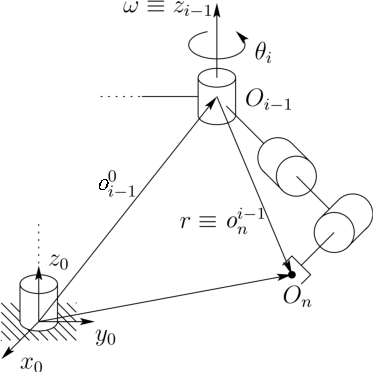
\includegraphics[width=0.5\linewidth]{./images/Effector_rotation}
\caption{Az $i$-edik ízület hatása a kéz sebességére}
\end{figure}

\subsection{A Jacobi-mátrix egyesítése}
A $J_v$ mátrixról szerzett eddigi ismereteinket összegezve a
\begin{equation}
J_{v} = [J_{v_{1}} J_{v_{2}} \ldots J_{v_{n}}]
\end{equation}
oszlopvektoros előállításra a
\begin{equation}
J_{v_{i}} = \begin{dcases*}
    z_{i-1} \times (o_{n} - o_{i-1}) & ha az $i$-edik ízület forgató\\
    z_{i-1} & ha az $i$-edik ízület eltoló
    \end{dcases*}
\end{equation}
összefüggés érvényes. Ehhez hasonlóan, a $J_{\omega}$ mátrix
\begin{equation}
J_{\omega} = [J_{\omega_{1}} J_{\omega_{2}} \ldots J_{\omega_{n}}]
\end{equation}
alakjára a
\begin{equation}
J_{\omega_{i}} = \begin{dcases*}
    z_{i-1} & ha az $i$-edik ízület forgató\\
    0 & ha az $i$-edik ízület eltoló
    \end{dcases*}
\end{equation}
eredményeket kaptuk. A két részt egyesítve \az+\eqref{eq:jacobidef} képlet szerint, egy $n$ ízületű robotkar 
Jacobi-mátrixát
\begin{equation}
J = [J_1 J_2 \ldots J_n]
\end{equation}
formában felírva, az $i$-edik oszlopra
\begin{equation}
J_i = \begin{bmatrix}
    z_{i-1} \times (o_{n} - o_{i-1}) \\ 
    z_{i-1}
    \end{bmatrix} 
\end{equation}
adódott, ha az $i$-edik ízület forgató, illetve
\begin{equation}
J_i = \begin{bmatrix}
    z_{i-1} \\ 
    0
    \end{bmatrix} 
\end{equation}
ha az $i$-edik ízület eltoló.

Vegyük észre, hogy ezek a kifejezések a Denavit-Hartenberg konvenció által meghatározott koordináta-rendszereket 
leíró mennyiségek. Ezért, ha ezeket már ismerjük, akkor a Jacobi-mátrixot már könnyedén ki tudjuk számolni belőlük. 
Valóban, a mátrix megadásához csupán a $z_i$ bázisvektorok és az $o_i$ origók koordinátáira van szükségünk. Mivel a 
direkt kinematikai feladat megoldása nélkülözhetetlen a robotkarok programozásához, ez azt jelenti, hogy egyúttal a 
direkt sebességkinematikai feladatot is megoldottuk.

Az előző fejezet eredményére visszaemlékezve könnyen meggondolható, hogy a $z_i$ vektor bázisrendszer szerinti 
koordinátáit a $T^{0}_{i}$ áttérési mátrix harmadik oszlopának első három eleme adja meg, az $o_i$ origó pedig a 
negyedik oszlop első három eleméből olvasható le. Tehát csak a $T$ mátrixok harmadik és negyedik oszlopára van 
szükségünk ahhoz, hogy a fenti formulák alapján kiszámoljuk a Jacobi-mátrixot.

Az itt leírt módszer azonban nem csak a kéz sebességének kiszámítására alkalmas, hanem a robotkar bármely 
tetszőleges pontjának sebességét megadhatjuk vele. Ez a mozgás dinamikai egyenleteinek felírásakor hasznos, amikor a 
szegmensek tömegközéppontjainak sebességeit kell meghatároznunk.

\section{Az analitikus Jacobi-mátrix}
Az előző szakaszban a robotkar geometriai tulajdonságaiból vezettünk le összefüggéseket a kéz sebességére 
vonatkozóan. Ennek megfelelően az így kapott mátrixot a geometriai Jacobi`=mátrixnak nevezzük. Ebben a 
konstrukcióban a kéz irányát egy forgatási mátrixszal, azaz kilenc paraméterrel adtuk meg. Most azt az esetet 
vizsgáljuk meg, amikor a koordináta-rendszer elfordulását három paraméterrel, azaz egy minimális reprezentációval 
írjuk le. Az ez alapján meghatározott $J_a(q)$ mátrixot az analitikus Jacobi-mátrixnak hívjuk. Jelölje mostantól
\begin{equation}
X = \begin{bmatrix}
    d(q) \\ 
    \alpha(q)
    \end{bmatrix} 
\end{equation}
a kéz helyzetét, ahol $d(q)$ a bázisrendszer origójából a kéz rendszerének origójába mutató vektor, $\alpha(q)$ 
pedig egy, a kéz bázisrendszerhez viszonyított elfordulását leíró minimális reprezentáció. Például legyen 
$\alpha = (\phi, \theta, \psi)^T$ Euler-szögekkel megadva. A geometriaihoz hasonlóan az analitikus Jacobi-mátrixra 
is felírható egy
\begin{equation} \label{eq:analdefi}
\dot{X} = 
    \begin{bmatrix}
    \dot{d} \\ 
    \dot{\alpha}
    \end{bmatrix} = J_a(q)\dot{q}
\end{equation}
alakú összefüggés a kéz sebességének meghatározására.

Megmutatható, hogy ha $R = R_{z, \psi} R_{y, \theta} R_{z, \phi}$ az Euler-szög transzformáció, azaz
\begin{equation}
R = \begin{bmatrix}
\mathrm{c}\psi \mathrm{c}\theta \mathrm{c}\phi - \mathrm{s}\psi \mathrm{s}\phi &  -\mathrm{c}\phi \mathrm{s}\psi - 
    \mathrm{c}\psi \mathrm{c}\theta \mathrm{s}\phi & \mathrm{c}\psi \mathrm{s}\theta \\
\mathrm{c}\psi \mathrm{s}\phi + \mathrm{c}\theta \mathrm{c}\phi \mathrm{c}\psi & \mathrm{c}\psi \mathrm{c}\phi - 
    \mathrm{c}\theta \mathrm{s}\psi \mathrm{s}\phi & \mathrm{s}\psi \mathrm{s}\theta \\
-\mathrm{c}\phi \mathrm{s}\theta & \mathrm{s}\theta \mathrm{s}\phi & \mathrm{c}\theta 
\end{bmatrix}
\end{equation}
ahol c és s a $\cos$ és $\sin$ rövidítése, akkor a hozzá tartozó $\omega$ szögsebesség a
\begin{equation} \label{eq:represent}
B(\alpha) = 
    \begin{bmatrix}
    \cos \psi \sin \theta & -\sin \psi & 0 \\ 
    \sin \psi \sin \theta & \cos \psi & 0 \\ 
    \cos \theta & 0 & 1
    \end{bmatrix} 
\end{equation}
jelölés használatával
\begin{equation}
\begin{aligned}
\omega &=
    \begin{bmatrix}
    \dot{\phi} \cos \psi \sin \theta - \dot{\theta} \sin \psi \\ 
    \dot{\psi} \sin \psi \sin \theta + \dot{\theta} \cos \psi \\ 
    \dot{\psi} \cos \theta + \dot{\psi}
    \end{bmatrix} = \\
&= \begin{bmatrix}
    \cos \psi \sin \theta & -\sin \psi & 0 \\ 
    \sin \psi \sin \theta & \cos \psi & 0 \\ 
    \cos \theta & 0 & 1
    \end{bmatrix} 
    \begin{bmatrix}
    \dot{\phi} \\ 
    \dot{\theta} \\ 
    \dot{\psi}
    \end{bmatrix} = B(\alpha)\dot{\alpha}
\end{aligned}
\end{equation}
formában áll elő. A fenti összefüggést egyesítve a Jacobi-mátrix korábbi
\begin{equation}
\begin{bmatrix}
v \\ 
\omega
\end{bmatrix} = J(q)\dot{q}
\end{equation}
definíciójával, azt kapjuk, hogy
\begin{equation}
J(q)\dot{q} = 
    \begin{bmatrix}
    v \\ 
    \omega
    \end{bmatrix} =
    \begin{bmatrix}
    \dot{d} \\ 
    B(\alpha)\dot{\alpha}
    \end{bmatrix}
\end{equation}
amit felírhatunk
\begin{equation}
\begin{bmatrix}
\dot{d} \\ 
B(\alpha)\dot{\alpha}
\end{bmatrix}
= \begin{bmatrix}
    I & 0 \\ 
    0 & B(\alpha)
    \end{bmatrix} 
    \begin{bmatrix}
    \dot{d} \\ 
    \dot{\alpha}
    \end{bmatrix}
\end{equation}
alakban is. Ekkor \az+\eqref{eq:analdefi} képletet behelyettesítve
\begin{equation}
\begin{bmatrix}
I & 0 \\ 
0 & B(\alpha)
\end{bmatrix} 
\begin{bmatrix}
\dot{d} \\ 
\dot{\alpha}
\end{bmatrix}
= \begin{bmatrix}
    I & 0 \\ 
    0 & B(\alpha)
    \end{bmatrix} J_a(q)\dot{q}
\end{equation}
adódik. Ezek alapján kaptunk egy módszert az analitikus Jacobi-mátrixnak a geometriaiból való kiszámítására
\begin{equation} \label{eq:geoanaljacobi}
J_a(q) = \begin{bmatrix}
    I & 0 \\ 
    0 & B(\alpha)^{-1}
    \end{bmatrix} J(q)
\end{equation}
módon, feltéve, hogy $\det B(\alpha) \neq 0$.

\section{Szingularitások meghatározása}
Azon konfigurációkat, melyekre a Jacobi-mátrix rangja nem maximális, szinguláris konfigurációknak vagy 
szingularitásoknak nevezzük. Ezeknek a vizsgálata az inverz sebességkinematika szempontjából fontos, mert látni 
fogjuk, hogy teljes rangú esetben a megoldás egyszerűen kiszámítható. 

További elnevezés még, hogy a $B(\alpha)$ mátrix szingularitásait reprezentációs szingularitásoknak hívjuk. 
\Az+\eqref{eq:represent} képletből könnyen megmutatható, hogy $\sin \theta \neq 0$ esetén $B(\alpha)$ invertálható, 
ami \az+\eqref{eq:geoanaljacobi} egyenlet szerint szükséges a teljes rangúsághoz. Ez ugyanis azt mutatja, hogy az 
analitikus Jacobi-mátrix szingularitásai magukban foglalják a reprezentáció és a geometriai Jacobi-mátrix 
szingularitásait.

A $6 \times n$-es $J(q)$ Jacobi-mátrix definíció szerint meghatároz egy
\begin{equation}
\xi = J(q)\dot{q}
\end{equation}
leképezést az ízületi sebességek $\dot{q}$ vektora és a kéz sebességének $\xi = (v, \omega)^T$ vektora között. Ez az 
összefüggés azt mutatja, hogy a kéz minden lehetséges sebességvektora a Jacobi-mátrix oszlopainak lineáris 
kombinációja, azaz részletesen kiírva
\begin{equation}
\xi = J_1 \dot{q}_1 + J_2 \dot{q}_2 + \cdots + J_n \dot{q}_n
\end{equation}
adódik. Mivel $\xi \in \mathbb{R}^6$, ezért szükséges, hogy $J$ oszlopai között legyen hat lineárisan független 
ahhoz, hogy a kéz tetszőleges sebességet el tudjon érni. Ez $6 < n$ esetén pontosan akkor teljesül, ha $J$ teljes 
rangú. Itt fontos megjegyezni, hogy ez a rang nem állandó, hanem a $q$ paraméterek függvényében változik.

A robotkar szingularitásainak azonosítása több okból is fontos feladat:
\begin{itemize}
\item A szingularitások olyan konfigurációkat jelölnek, melyekből a kéz bizonyos irányú mozgásai nem valósíthatóak 
    meg, azaz a robotkar veszít a szabadsági fokából.
\item Szingularitásoknál korlátos kéz-sebességekhez nem korlátos ízületi sebességek tartozhatnak, mert ezek 
    kiolthatják egymást.
\item Szingularitásoknál a kézre vonatkozó korlátos erőkhöz és nyomatékokhoz nem korlátos ízületi erők és nyomatékok 
    tartozhatnak.
\item A szingularitások általában a robot munkaterének peremén, azaz a hatósugarának szélén lévő pontokhoz 
    tartoznak, hiszen ezeknél messzebbre nem juttatható el a kéz.
\item A szingularitások a munkatér azon pontjaihoz tartoznak, melyek elérhetetlenné válnak a robotkar alaki 
    tulajdonságainak tetszőlegesen kicsi megváltoztatása esetén. Ez a terhelés által bekövetkező esetleges 
    deformálódások miatt fontos.
\item Szingularitások közelében nem létezik egyértelmű megoldása az inverz kinematikai problémának. Ilyen esetekben 
    vagy nincs megoldás, vagy végtelen sok van.
\end{itemize}

Számos módszer létezik a Jacobi-mátrix szingularitásainak meghatározására. Mi a $J(q) \in \mathbb{R}^{6 \times 6}$ 
esetben azt a tényt fogjuk kihasználni, hogy egy négyzetes mátrix pontosan akkor szinguláris, ha a determinánsa 
nulla. Általában egy $\det J(q) = 0$ nemlineáris egyenlet megoldása nehéz feladat. Egy eljárás, amely ebben 
segítségünkre lehet, az a szingularitások szétbontásának módszere. Ez minden olyan esetben használható, amikor a 
robotkar például gömbcsuklóval van felszerelve.

\subsection{Szingularitások szétbontása}
Az eddigiekben a robotkar helyzetét a szegmensekhez rögzített koordináta`=rendszerek segítségével határoztuk meg, a 
direkt kinematikai feladat megoldása által. Vegyük észre, hogy a Denavit-Hartenberg konvenció csupán egy 
szisztematikus módszer ennek elvégzésére. Habár az így kapott egyenletek függenek a koordináta-rendszerek 
megválasztásától, maga a robotkar konfigurációja egy geometriai mennyiség, amely független az őt leíró 
koordináta-rendszerektől. Ennek felismerésével lehetőség nyílik számunkra, hogy gömbcsuklóval felszerelt robotkarok 
esetén a szingularitások vizsgálatát szétbontsuk két egyszerűbb problémára. Az első az úgynevezett 
kar-szingularitások meghatározása, melyek a kar, azaz az első három vagy több ízület mozgásából adódnak. A második a 
csukló-szingularitások meghatározása, melyek a gömbcsukló mozgásából erednek.

Tegyük fel, hogy $n = 6$, azaz a manipulátor egy három szabadságfokú karból és egy három szabadságfokú gömbcsuklóból 
áll. Ekkor a Jacobi-mátrix egy $6 \times 6$-os mátrix, és egy $q$ konfiguráció pontosan akkor szinguláris, ha 
$\det J(q) = 0$.

Bontsuk fel a Jacobi-mátrixot a karhoz és a gömbcsuklóhoz tartozó részre, majd particionáljuk tovább $3 \times 3$-as 
blokkokra
\begin{equation}
J = [J_P | J_O] = \left[ \begin{array}{c|c}
    J_{11} & J_{12} \\ 
    \hline
    J_{21} & J_{22}
    \end{array} \right]
\end{equation}
módon. A forgató ízületekre kapott összefüggés alapján az utolsó három ízületre
\begin{equation}
J_O = \begin{bmatrix}
    z_3 \times (o_6 - o_3) & z_4 \times (o_6 - o_4) & z_5 \times (o_6 - o_5) \\ 
    z_3 & z_4 & z_5
    \end{bmatrix} 
\end{equation}
A gömbcsukló tengelyei egy közös pontban metszik egymást, ezért ha úgy választjuk meg a koordináta-rendszereket, 
hogy $o_3 = o_4 = o_5 = o_6 = o$ teljesüljön, akkor
\begin{equation}
J_O = \begin{bmatrix}
    0 & 0 & 0 \\ 
    z_3 & z_4 & z_5
    \end{bmatrix} 
\end{equation}
alakú lesz. Ez azért hasznos, mert ekkor a Jacobi-mátrix blokkjai alsó háromszögmátrixot alkotnak
\begin{equation}
J =\begin{bmatrix}
    J_{11} & 0 \\ 
    J_{21} & J_{22}
    \end{bmatrix} 
\end{equation}
formában, melynek determinánsa
\begin{equation}
\det J = \det J_{11} \det J_{22}
\end{equation}
ahol $J_{11}$ és $J_{22}$ $3 \times 3$-as mátrixok. Itt a $J_{11}$ mátrix $i$-edik oszlopa 
$z_{i-1} \times (o - o_{i-1})$, ha az $i$-edik ízület forgató, illetve $z_{i-1}$, ha az ízület eltoló, továbbá 
$J_{22} = [z_3, z_4, z_5]$.

Tudjuk, hogy $\det J = 0$ pontosan akkor teljesül, ha $\det J_{11} = 0$ vagy $\det J_{22} = 0$. Ezek közül az első 
egyenletet a kar, a másodikat pedig a gömbcsukló szingularitásai elégítik ki. Ezzel azt kaptuk, hogy a manipulátor 
szinguláris konfigurációinak halmaza a két egyenlet megoldáshalmazainak uniója. Fontos megjegyezni, hogy a 
Jacobi-mátrix ezen alakja nem szükségképpen adja meg a helyes összefüggést a kéz sebessége és az ízületi sebességek 
között, csupán a szingularitások meghatározásának egyszerűsítését szolgálja.

\begin{figure}[h]
\centering
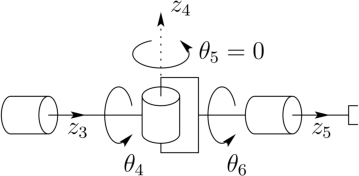
\includegraphics[width=0.5\linewidth]{./images/Wrist_singularity}
\caption{A gömbcsukló szingularitása}
\end{figure}

Az előző egyenletekből azt kaptuk, hogy egy gömbcsukló pontosan akkor van szinguláris konfigurációban, ha a 
$z_3, z_4$ és $z_5$ vektorok lineárisan összefüggőek. Ez akkor fordulhat elő, amikor a $z_3$ és a $z_5$ tengelyek 
egy egyenesbe esnek. Minden olyan konfiguráció, amelyben két forgató ízület tengelye egybeesik, szingularitást 
eredményez, mivel ekkor egyenlő nagyságú, de ellentétes irányú forgatások nem változtatják meg a kéz helyzetét. 
A fenti konfiguráció a gömbcsukló egyetlen szingularitása, és ez a geometriai felépítése miatt elkerülhetetlen. 
A kar-szingularitások az adott manipulátorhoz tartozó $J_{11}$ mátrix kiszámítása után $\det J_{11} = 0$ 
megoldásával könnyen meghatározhatóak.

Ez a feladat elsősorban az útvonalkeresés szempontjából fontos. Olyan görbe mentén szeretnénk mozgatni a robot 
kezét, amely vagy elkerüli a szingularitásokat, vagy olyan irányban halad át rajtuk, amelyre létezik egyértelmű 
megoldás.

\begin{figure}[h]
\centering
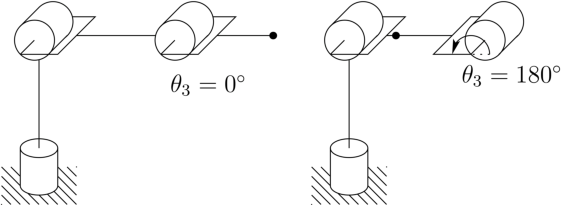
\includegraphics[width=0.6\linewidth]{./images/Elbow_singularity}\hspace{0.2cm}
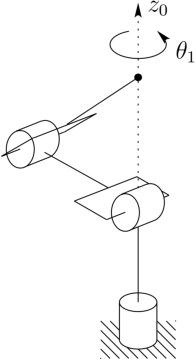
\includegraphics[width=0.2\linewidth]{./images/Shoulder_singularity}
\caption{Az antropomorf robotkar szingularitásai}
\end{figure}

\section{Az inverz sebességkinematikai feladat}
Korábban említettük az inverz sebességkinematikai problémát, melynek kiindulópontja az
\begin{equation}
\xi = J\dot{q}
\end{equation}
egyenlet, amely az ízületek $\dot{q}$ sebességgel történő mozgásából eredő kéz-sebességet adja meg. Az inverz  
feladat célja, hogy megtalálja azon $\dot{q}$ ízületi sebességeket, melyekre adott $\xi$ esetén a fenti összefüggés 
teljesül, azaz amelyekre kéz az előírt $\xi$ sebességvektorral mozog. Ha a Jacobi-mátrix négyzetes és nem 
szinguláris, akkor ez a probléma egyszerűen megoldható egy invertálással, hiszen
\begin{equation}
\dot{q} = J^{-1}\xi
\end{equation}

Azon manipulátorok esetében, amelyek nem pontosan hat ízületből állnak, a Jacobi-mátrix nem invertálható, hiszen nem 
is négyzetes. Ebben az esetben az inverz feladat pontosan akkor oldható meg, ha $\xi$ benne van a $J$ oszlopai által 
kifeszített térben. Ez egyszerűen eldönthető a következő rangvizsgálattal, amelyet lineáris algebrából ismerünk. 
\begin{áll}
Egy $\xi$ vektor akkor és csak akkor van benne egy $J(q)$ mátrix képterében, ha 
$\mathrm{rang}J(q) = \mathrm{rang}[J(q) | \xi]$.
\end{áll}
Ennek megoldására számos algoritmus létezik, például az egyik ilyen a Gauss-elimináció. 

Van azonban egy érdekes módszer abban az esetben, amikor $n > 6$. Ekkor a $\dot{q}$ megoldást $J$ jobb oldali 
pszeudoinverze segítségével is megkaphatjuk. 
\begin{defi}
Legyen $m < n$. Ekkor egy $J \in \mathbb{R}^{m \times n}$ mátrix jobb oldali pszeudoinverzén azt a $J^+$ mátrixot 
értjük, melyre $JJ^+ = I$, ahol $I \in \mathbb{R}^{m \times m}$.
\end{defi}
Ezen pszeudoinverz megkonstruálásához felhasználjuk a lineáris algebra alábbi eredményét.
\begin{áll}
Minden $J \in \mathbb{R}^{m \times n}$ mátrixra, ha $m < n$ és $\mathrm{rang}J = m$, akkor a $(JJ^T)$ mátrixnak 
létezik inverze.
\end{áll}
Ebben az esetben $(JJ^T) \in \mathbb{R}^{m \times m}$, és $\mathrm{rang}(JJ^T) = m$. Ekkor az állítás értelmében 
felírható a
\begin{equation}
(JJ^T)(JJ^T)^{-1} = I
\end{equation}
egyenlet, amelyből átzárójelezéssel
\begin{equation}
\begin{aligned}
J \left(J^T (JJ^T)^{-1} \right) &= I \\
JJ^+ &= I
\end{aligned}
\end{equation}
adódik. A fenti kifejezésben a $J^+ = J^T (JJ^T)^{-1}$ mátrixot $J$ jobb oldali pszeudoinverzének nevezzük, mivel 
eleget tesz a definíciónak, azaz $JJ^+ = I \in \mathbb{R}^{m \times m}$. Vegyük észre, hogy 
$J^+ J \in \mathbb{R}^{n \times n}$, és általában $J^+ J \neq I$. 

Innen már könnyen belátható, hogy egy megoldást szolgáltat a
\begin{equation}
\dot{q} = J^+ \xi + (I - J^+ J)b
\end{equation}
kifejezés, ahol $b \in \mathbb{R}^n$ tetszőleges vektor. Ennek igazolásához egyszerűen csak be kell helyettesíteni 
\az+\eqref{eq:jacobidef} egyenletbe, azaz szorozzuk be balról mindkét oldalt $J$-vel.
\begin{equation}
\begin{aligned}
J\dot{q} &= J \left(J^+ \xi + (I - J^+ J)b \right) = \\
    &= JJ^+ \xi + J(I - J^+ J)b = \\
    &= JJ^+ \xi + (J - JJ^+ J)b
\end{aligned}
\end{equation}
Kihasználva, hogy $J^+$ pszeudoinverze $J$-nek, azt kapjuk, hogy
\begin{equation}
\begin{aligned}
JJ^+ \xi + (J - JJ^+ J)b = \xi + (J - J)b = \xi
\end{aligned}
\end{equation}

Általában, $m < n$ esetén $(I - J^+ J) \neq 0$, és minden $(I - J^+ J)b$ alakú vektor $J$ nullterében van. Ez azt 
jelenti, hogy ha $\dot{g}$ az ízületi sebességek egy olyan vektora, amely $\dot{g} = (I - J^+ J)b$ alakú, akkor 
$J\dot{g} = 0$, vagyis az ízületek $\dot{g}$ sebességgel történő mozgatása esetén a kéz egy helyben marad. Ezért, ha 
$\dot{q}$ egy megoldás, akkor $\dot{q} + \dot{g}$ is megoldás minden $\dot{g} = (I - J^+ J)b$ esetén, ahol $b$ 
tetszőleges vektor. 

A $J$ mátrix jobb oldali pszeudoinverze egyszerűen megkapható a szinguláris értékek szerinti felbontásából.
\begin{áll}
Minden $J \in \mathbb{R}^{m \times n}$ mátrix felbontható $J = U\Sigma V^T$ alakban, ahol 
$U \in \mathbb{R}^{m \times m}$ és $V \in \mathbb{R}^{n \times n}$ ortogonális mátrixok, 
$\Sigma \in \mathbb{R}^{m \times n}$ pedig a szinguláris értékek mátrixa.
\end{áll}
Ekkor a pszeudoinverz felírható
\begin{equation}
J^+ = V\Sigma^+ U^T
\end{equation}
alakban, ahol $U$ és $V$ ortogonális mátrixok,
\begin{equation}
\Sigma^+ = 
    \left[ \begin{array}{c}
    \begin{array}{ccc}
    \sigma^{-1}_{1} &  &  \\ 
     & \ddots &  \\ 
     &  & \sigma^{-1}_{m}
    \end{array}  \\
    \hline 
    0
    \end{array} \right]
\end{equation}
pedig a szinguláris értékek inverzeinek $n \times m$-es mátrixa.

Hasonló módszert alkalmazhatunk akkor is, amikor az analitikus Jacobi-mátrixot használjuk a geometriai helyett. 
Az ízületi sebességek és a kéz sebessége közötti kapcsolatot az analitikus Jacobi-mátrix \az+\eqref{eq:analdefi} 
egyenlet alapján
\begin{equation} \label{eq:analjacobi}
\dot{X} = J_a(q)\dot{q}
\end{equation}
formában adja meg. Tehát az inverz sebességkinematikai feladat ismét egy lineáris egyenletrendszer megoldására 
vezethető vissza, amely az előzőekhez hasonlóan oldható meg.

\Az+\eqref{eq:analjacobi} egyenletet még egyszer deriválva kapjuk az
\begin{equation}
\ddot{X} = J_a(q)\ddot{q} + \diff{}{t} \big( J_a(q) \big) \dot{q}
\end{equation}
gyorsulási egyenletet. Ez alapján, ha adott a kéz gyorsulásának $\ddot{X}$ vektora, akkor az ízületek pillanatnyi 
gyorsulásának $\ddot{q}$ vektorát a
\begin{equation}
b = \ddot{X} - \diff{}{t} \big( J_a(q) \big) \dot{q} = J_a(q)\ddot{q}
\end{equation}
egyenlet megoldásából kapjuk.

A hat szabadságfokú manipulátorokra alkalmazva a fentieket, az inverz sebesség- és gyorsulásegyenletek
\begin{equation}
\dot{q} = J_a(q)^{-1}\dot{X}
\end{equation}
valamint
\begin{equation}
\ddot{q} = J_a(q)^{-1}b
\end{equation}
alakban írhatóak fel, feltéve, hogy $\det J_a(q) \neq 0$.

\chapter{Összefoglalás}
Az előző fejezetekben azokra a kérdésekre kerestük a választ, hogy hogyan határozhatjuk meg a manipulátor kezének 
pozícióját, orientációját, lineáris illetve szögsebességét, valamint hogy milyen ízületi paraméterek segítségével 
érhető el, hogy a kéz adott helyzetbe kerüljön, vagy hogy adott sebességgel mozogjon. Ezek megválaszolása érdekében 
bevezettük a Denavit-Hartenberg konvenciót, amellyel könnyen le tudtuk írni a szegmensekhez illesztett 
koordináta-rendszerek helyét és elfordulását, azaz megoldottuk a direkt kinematikai feladatot. 

A sebességkinematikai probléma keretében megismerkedtünk a ferdén szimmetrikus mátrixokkal, a szögsebességgel és 
ezeknek a forgatási mátrixokhoz való viszonyával. Levezettünk néhány képletet az eredő lineáris és szögsebesség 
kiszámítására. Ennek segítségével meghatároztuk a robotkar Jacobi-mátrixát, amellyel a kéz sebességét már könnyen 
meg tudtuk adni. Ezek után megvizsgáltuk a manipulátor szingularitásait, azaz azon konfigurációkat, melyekre a kar 
veszít a szabadságfokából. Végül megoldottuk az inverz sebességkinematikai feladatot, melynek eredményeképpen 
tetszőleges sebességgel és gyorsulással tudtuk mozgatni a robot kezét.

\nocite{*}

\DeclareNameAlias{default}{last-first}
\renewbibmacro*{name:last-first}[4]{%
  \ifuseprefix
    {\usebibmacro{name:delim}{#3#1}%
     \usebibmacro{name:hook}{#3#1}%
     \ifblank{#3}{}{%
       \ifcapital
         {\mkbibnameprefix{\MakeCapital{#3}}\isdot}
     {\mkbibnameprefix{#3}\isdot}%
       \ifpunctmark{'}{}{\bibnamedelimc}}%
     \mkbibnamelast{#1}\isdot
     \ifblank{#4}{}{\bibnamedelimd\mkbibnameaffix{#4}\isdot}%
%      \ifblank{#2}{}{\addcomma\bibnamedelimd\mkbibnamefirst{#2}\isdot}}% DELETED
     \ifblank{#2}{}{\bibnamedelimd\mkbibnamefirst{#2}\isdot}}% NEW
    {\usebibmacro{name:delim}{#1}%
     \usebibmacro{name:hook}{#1}%
     \mkbibnamelast{#1}\isdot
     \ifblank{#4}{}{\bibnamedelimd\mkbibnameaffix{#4}\isdot}%
%      \ifblank{#2#3}{}{\addcomma}% DELETED
     \ifblank{#2}{}{\bibnamedelimd\mkbibnamefirst{#2}\isdot}%
     \ifblank{#3}{}{\bibnamedelimd\mkbibnameprefix{#3}\isdot}}}
     
\renewcommand\mkbibnamelast[1]{\textsc{#1}}

\printbibliography
\end{document}